\documentclass{../industrial-development}
\graphicspath{{11-IT-specialist's-way/}}

\title{ Лекция №\,11 по теме «Путь специалиста в ИТ---индустрии»}
\author{ПИ---21МО Шогина Мария}
\date{2017 }


\begin{document}

\begin{frame}
  \titlepage
\end{frame}

\section{Варианты трудоустройства }

\subsection{}

\begin{frame} \frametitle{Варианты трудоустройства}
  \begin{block}{}
  Существует множество способов выгодно применять ваши навыки разработчика ПО 

Особо стоит отметить 3 варианта трудоустройства, такие как:
  \end{block}
  
  \begin{itemize}
  \item Служащий
  \item Независимый консультант
  \item Предприниматель
  \end{itemize}
\end{frame}

\lecturenotes
 Существует~\cite[с.~62--67]{Sonmez} множество способов выгодно применять ваши навыки разработчика ПО. Особо стоит отметить 3 варианта трудоустройства, такие как:
Служащий
 Независимый консультант
Предприниматель
Далее о плюсах и минусах каждого подробнее.

\begin{frame} \frametitle{Варианты трудоустройства: Служащий}
  \begin{block}{}
    Выбор места работы, который делает большинство разработчиков ПО 
  \end{block}
  
  \centerline{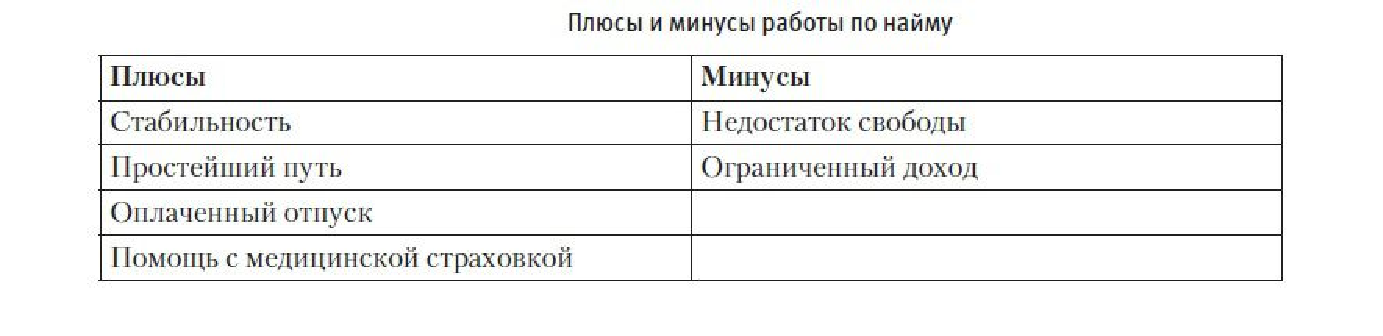
\includegraphics[height=0.38\textheight]{11-IT-specialist's-way/sl.pdf}}
\end{frame}

\lecturenotes
Стандартный~\cite[с.~62--67]{Sonmez} и очевидный выбор места работы, который делает большинство разработчиков ПО. 
Самый большой плюс — стабильность. Под стабильностью подразумевается, что у вас постоянный источник зарабатывания денег. Если вы выбрали быть служащим, то до тех пор, пока у вас есть работа, у вас будет зарплата. В будущем есть вероятность  потерять эту работу и придется искать новую, но пока у вас период относительной стабильности, когда можно рассчитывать на определенный доход каждый месяц.
Вариант «быть служащим» также является самым простым из доступных, поскольку ваша ответственность будет ограниченна, а путь — довольно очевиден. Процесс поиска работы и трудоустройства хорошо поставлен. Вам не придется определять, что же нужно сделать, чтобы вам заплатили. У вас также будет оплачиваемый отпуск и — по крайней мере в Соединенных Штатах — помощь с медицинской страховкой.
Негативная сторона работы по найму затрагивает вашу свободу. Как служащий, вы должны тратить большую часть времени на то, чтобы решать задачи для вашего работодателя. Вы практически никак не можете повлиять на то, какую работу нужно делать, и не всегда будете делать то, что нравится. Скорее всего, также придется соблюдать расписание: сколько часов в неделю вы должны работать.
Несмотря на то что ваш доход известен заранее, он, скорее всего, будет иметь верхнюю границу. Будучи служащим, вы в конце концов достигнете потолка доходов и возможностей продвижения по карьерной лестнице.


\begin{frame} \frametitle{Варианты трудоустройства: Независимый консультант}
  \begin{block}{}
    Независимый консультант --- это разработчик ПО, который не работает на конкретного работодателя 
  \end{block}
  
    \centerline{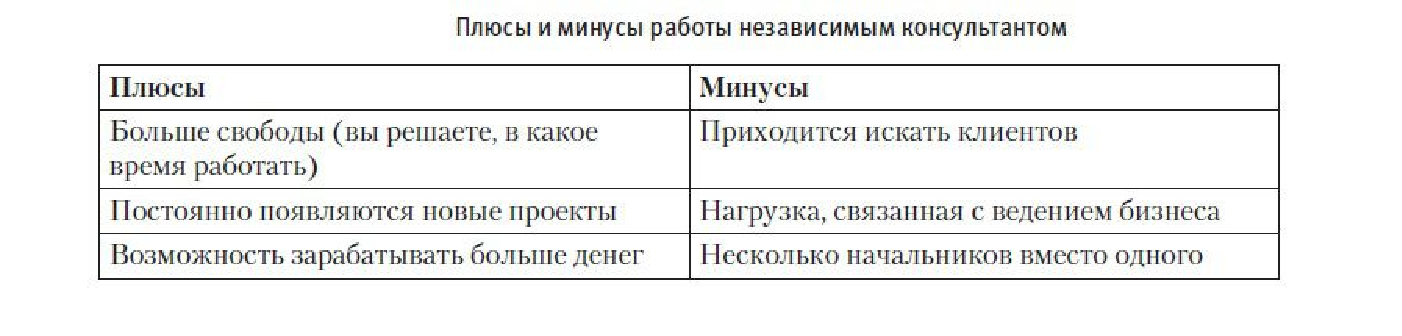
\includegraphics[height=0.38\textheight]{11-IT-specialist's-way/fl.pdf}}
\end{frame}

\lecturenotes
Многие~\cite[с.~62--67]{Sonmez} разработчики ПО зарабатывают на жизнь независимыми консультантами. Независимый консультант — это разработчик ПО, который не работает на конкретного работодателя. Вместо этого у него один или несколько клиентов. Если у вас когда-нибудь была работа на стороне, когда вы программировали для клиента, который оплачивал труд по часам (или сумма была заранее оговоренной), вы знаете, что значит быть консультантом.
Разработчик считается независимым консультантом, если он получает большую часть своего дохода подобным образом. Консультант отличается от разработчика ПО, работающего по контракту, поскольку последний трудится только на одного  клиента. Работа по контракту ближе к работе по найму. Независимый консультант обычно имеет собственную компанию, которая заключает контракты на выполнение работ, но при этом он не привязан к одному клиенту.
Нельзя сказать, что профессия независимого консультанта имеет сплошные минусы. В том, что вы отчитываетесь не одному работодателю, есть и плюсы. Как независимый консультант вы можете самостоятельно определять рабочие часы, а также работу, за которую будете браться. Вы можете приходить и уходить в любое время и составлять гибкое расписание, но клиенты будут ожидать от вас того, что работа будет выполнена своевременно.
Самый большой плюс — это, скорее всего, потенциальный заработок. Как независимый консультант вы можете получать в час гораздо больше, чем работая на кого-то. 
Несмотря на то что может показаться, что работа независимым консультантом приносит немалый доход, много времени уходит на поиск клиентов и прочие задачи, связанные с управлением бизнесом. Если вы независимый консультант, то фактически являетесь бизнесом (не только в ваших мыслях). Вы отвечаете за уплату налогов, юридические вопросы, продажи, здоровье и все остальное, что связано с ведением бизнеса.


\begin{frame} \frametitle{Варианты трудоустройства: Предприниматель}
  \begin{block}{}
 Путь предпринимателя самый трудный, самый неопределенный и потенциально самый прибыльный
  \end{block}
  
  \centerline{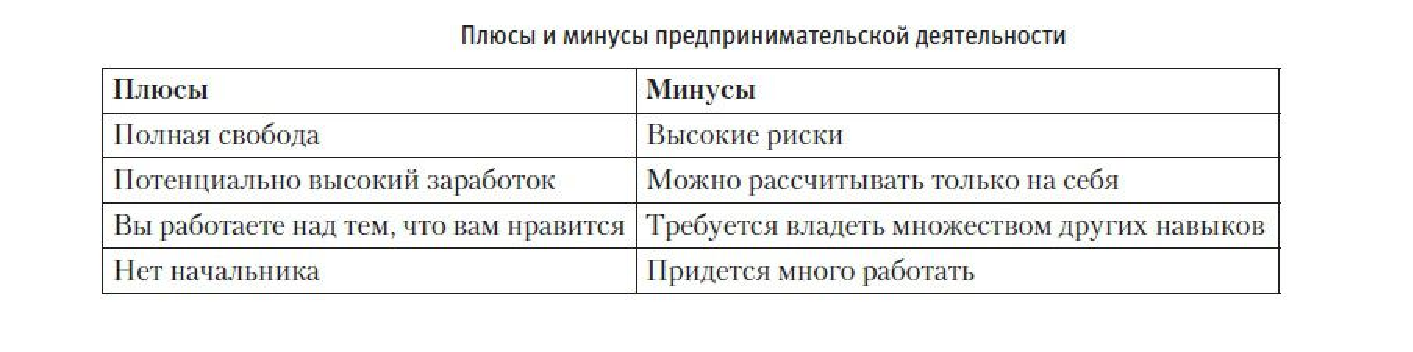
\includegraphics[height=0.39\textheight]{11-IT-specialist's-way/pr.pdf}}
\end{frame}

\lecturenotes
Путь~\cite[с.~62--67]{Sonmez} предпринимателя, возможно, самый трудный, самый неопределенный и потенциально самый прибыльный. Этому есть объяснение. Этот вариант не несет никакой стабильности, но если вам повезет, то по-крупному.
Определение этого пути довольно расплывчатое и может значить множество разных вещей. Разработчика считается предпринимателем, если он развивает свой бизнес или продукт с использованием профессиональных навыков. В то время как служащий и независимый консультант меняют свое время на деньги, предприниматель меняет свое время не на моментальную выручку, а на шанс получить высокую оплату в будущем.
Разработчики-предприниматели создают стартапы и ищут финансирование у внешних инвесторов, которое называется венчурным капиталом. Или открывают маленькие компании, работающие по принципу «программа как служба» (software-as-a-service, SaaS), и зарабатывают деньги, продавая подписки на их службу. Например, основатели популярной службы по обучению разработчиков Pluralsight начали с обучения людей в кабинетах. Но позднее поняли, что могут улучшить качество услуг, перенеся обучение в Интернет, поэтому перешли к модели SaaS и начали предлагать службу, основанную на подписке.
Я уверен, что вы теперь самостоятельно можете определить два самых больших преимущества предпринимательской деятельности: полная свобода и неограниченные возможности заработка. У вас не будет начальника, кроме самого. Вы можете приходить на работу и уходить когда вздумается, вы полностью отвечаете за свое будущее. Вы также можете зарабатывать миллионы долларов, если создадите очень успешный продукт. Кроме того, если правильно вложиться в собственное время, то ваши доходы от этого могут вырасти экспоненциально.
Но предпринимательская деятельность включает в себя риск. Доход совершенно не гарантирован, и вы можете залезть в долги, пытаясь реализовать свои гениальные идеи. Жизнь предпринимателя похожа на американские горки. В один день у вас есть покупатели — и вы чувствуете, будто находитесь на вершине мира. На следующий день о проекте забывают — и вам приходится ломать голову, как оплатить счета.
Предпринимательство также требует от вас развития навыков, о которых не нужно беспокоиться, если вы работаете на кого-то или являетесь независимым консультантом. Предприниматели должны изучить продажи, маркетинг, а также другие аспекты ведения бизнеса и финансов, которые являются важными составляющими успеха. 

%\section{}

\section{Возможные пути развития специалиста. }

\subsection{2.1 Развитие  специалиста по ступеням профессионального мастерства. }


\subsection{}

\begin{frame} \frametitle{Развитие  специалиста по ступеням профессионального мастерства}
  \begin{block}{}
  По мере того как вы приобретаете более соответствующий опыт работы, вы можете постепенно занимать более высокие позиции

 Выделяют 4 основных позиций:
  \end{block}
  
  \begin{itemize}
  \item Младший(Стажер) --- Junior
  \item Старший --- Middle
  \item Ведущий --- Senior
 \item Главный --- Lead
  \end{itemize}
\end{frame}

\lecturenotes
 По мере того как вы приобретаете более соответствующий опыт работы, вы можете постепенно занимать более высокие позиции. Выделяют 4 основных позиций~\cite{JMSL}:

Младший(Стажер) --- Junior
Старший --- Middle
Ведущий --- Senior
 Главный --- Lead
Официальная градация, пропагандируемая работными сайтами~\cite{hh}, и на которую ориентируется большинство, выглядит так:
	0,5-1,5 года реального опыта = Junior
	1-3 года = Middle 
	4-6 лет = Senior
	>6 лет = Lead


\begin{frame} \frametitle{Развитие  специалиста по ступеням профессионального мастерства}
 \centerline{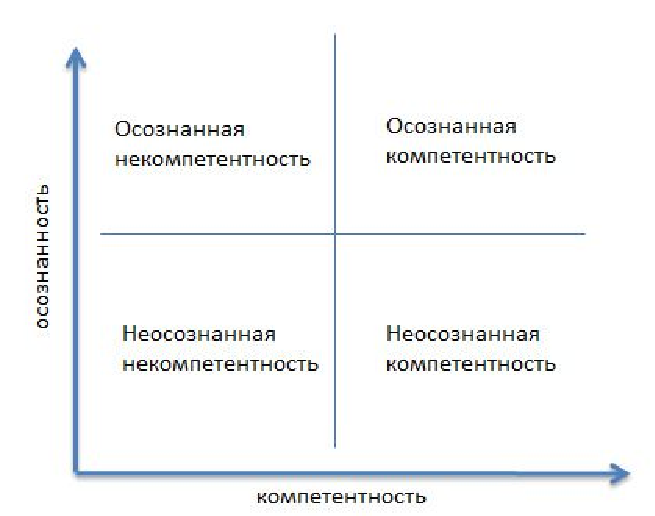
\includegraphics[width=0.54\linewidth]{11-IT-specialist's-way/matrix.pdf}}
  \begin{itemize}
  \item Младший(Стажер) --- в квадрате «Неосознанная некомпетентность»
  \item Старший  --- в квадрате «Осознанная некомпетентность»
  \item Ведущий --- в квадрате «Осознанная компетентность»
 \item Главный --- в квадрате «Неосознанная компетентность»
  \end{itemize}
\end{frame}

\lecturenotes
Junior~\cite{JMSL}
Люди на этой позици, не могут представить объем работы в той или иной области, ответственности. Многие находятся в квадрате «Неосознанная некомпетентность» по многим своим навыкам. Люди, процентное понимание области которых примерно 0 - 25%. 
Middle 
Навыки, которые были у junior на уровне 0 – 25, на этом этапе перейдут в 25 – 50%. По факту: для многих навыков фокус сместится в “Осознанную некомпетентность”. Появление практической базы навыков. Таким образом, то, что знал junior на базовом уровне, middle уже знает более глубоко, но все же еще не эксперт в этой области. 
Senior
Многие вещи оказываются в квадрате «осознанная компетентность». В этом квадрате навыки, в которых вы уже реально разбираетесь и умеете применить на практике, а также можете объяснить другим. Человек выступает как консультант по этим навыкам, у него многогранный опыт в этой области.
Lead
По факту: для многих навыков фокус сместится в “Неосознанную компетентность”.Lead это Senior к обязанностям которого добавляются еще и обязанности по управлению командой, формирования стратегий развития, контролю исполнения бизнес-процессов. Контролирует работу нижестоящего персонала, обучает новичков.


%\section{}

\subsection{2.2 Развитие  специалиста в иерархии компании.  }

\subsection{}

\begin{frame} \frametitle{Развитие  специалиста в иерархии компании: Полная схема }
  \centerline{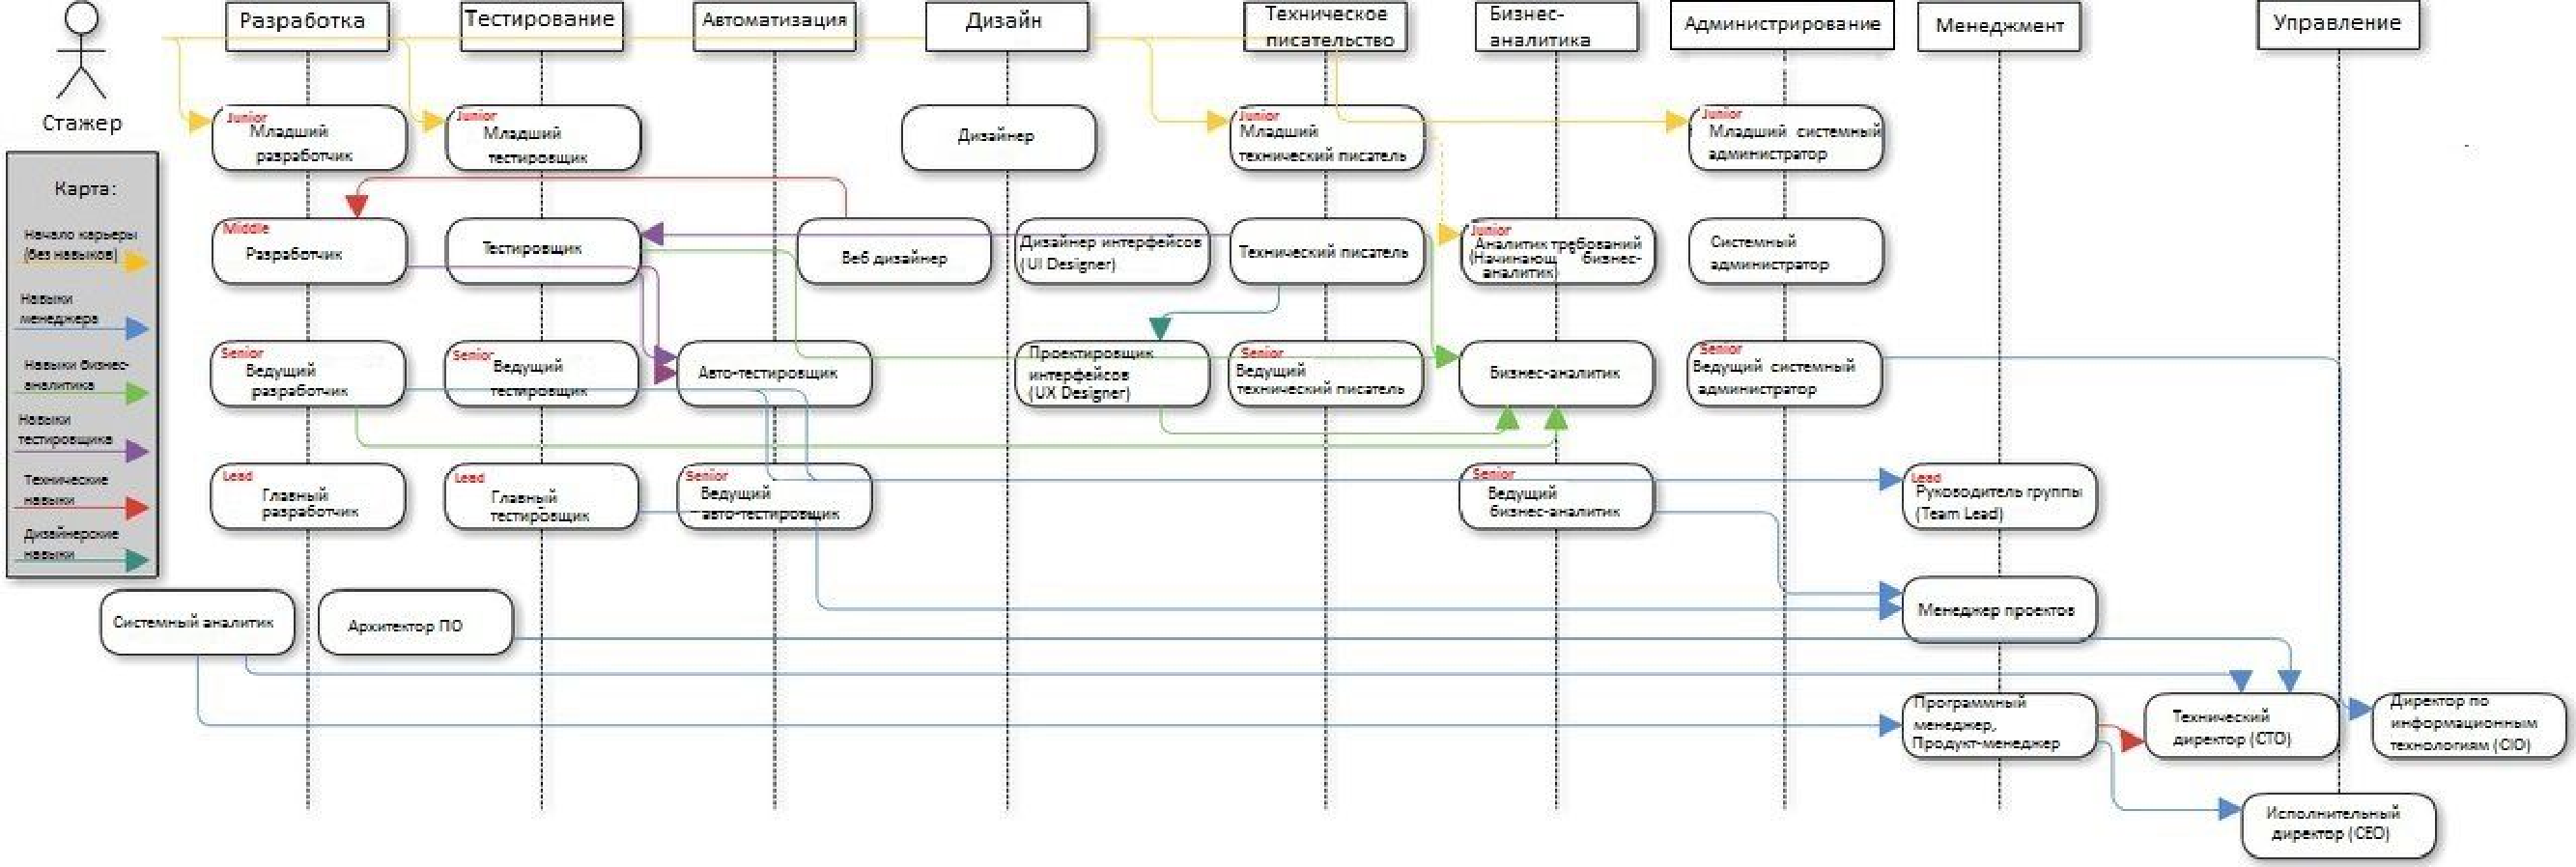
\includegraphics[height=0.47\textheight]{11-IT-specialist's-way/sch.pdf}}
\end{frame}

\lecturenotes
Развитие  специалиста по ступеням профессионального мастерства безусловно важно, так как влечет за собой и развитие специалиста в иерархии компании.
Так~\cite{mc} выглядит полная схема развития специалиста в иерархии компании.Анализ схемы начнется с позиции- стажера. Также  будут рассмотрены прямые и косвенные ветки перехода между различными сегментами внутри ит рынка. Карта схемы поможет более быстро и легко разбираться в косвенных ветках.Имеет смысл рассматривать данную схему более подробно по частям.

\begin{frame} \frametitle{Развитие  специалиста в иерархии компании: 1 часть из 4 }
  \centerline{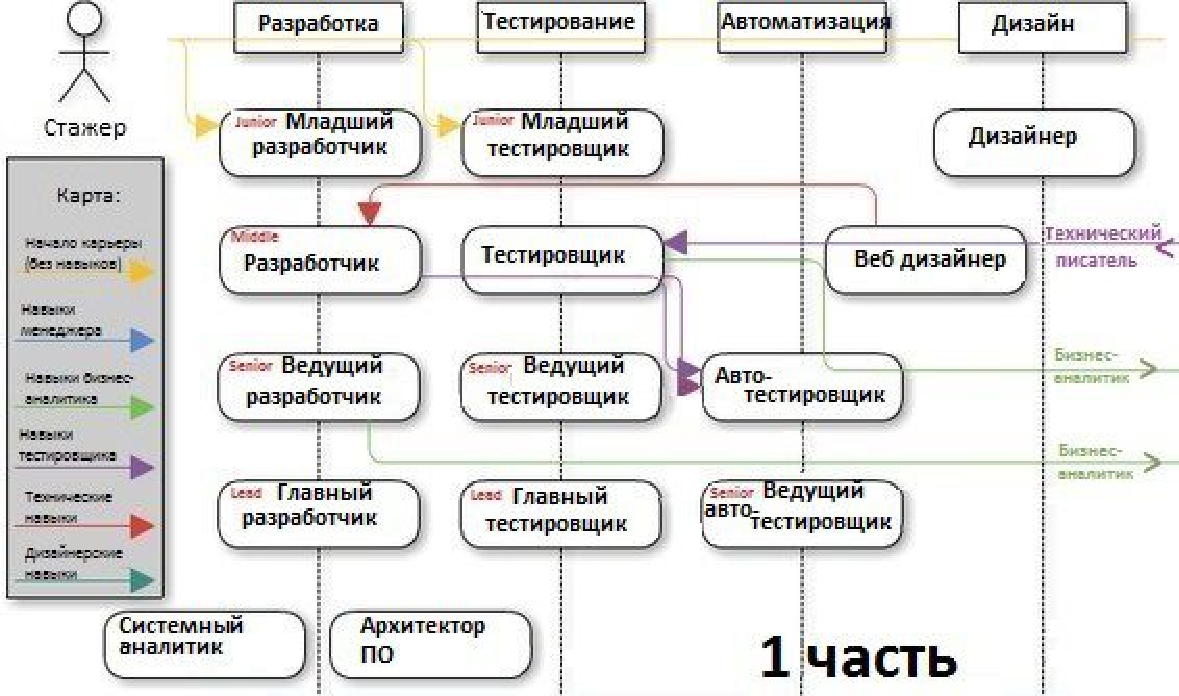
\includegraphics[width=1\linewidth]{11-IT-specialist's-way/sch11.pdf}}
\end{frame}

\lecturenotes
В 1 части оказались 4 сегмента ит рынка, такие как: Разработка,Тестирование, Автоматизация и Дизайн.
Прмые ветки:
1) 1ой прямой веткой --- является ветки внутри сегмента, связанного с разработкой
2) 2ой прямой веткой  --- является ветки внутри сегмента, связанного с тестированием
3) 3ей прямой веткой --- является ветки внутри сегмента, связанного с автоматизацией
4)4ой прямой веткой --- является ветки внутри сегмента, связанного с дизайном.( не является полной, продолжение данной ветки находится на 2 часте схемы).

\begin{frame} \frametitle{Прямая ветка разработчика}
 \centerline{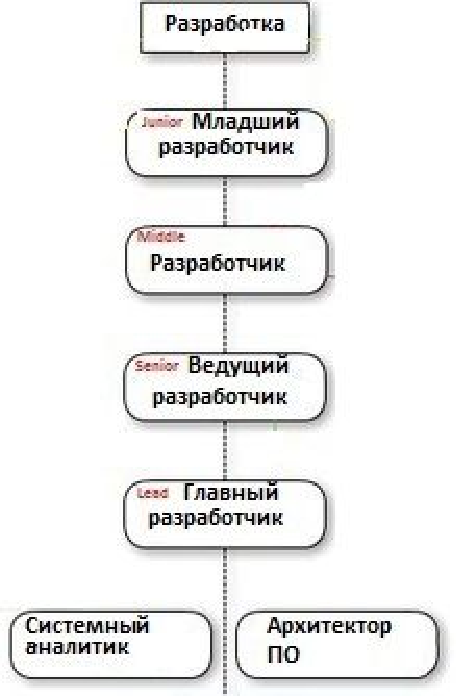
\includegraphics[width=0.46\linewidth]{11-IT-specialist's-way/sch11a.pdf}}
\end{frame}

\lecturenotes
 1ой~\cite{mc} прямой веткой --- является ветка внутри сегмента, связанного с разработкой. Далее рассмотрим подробнее

\begin{frame} \frametitle{Прямая ветка разработчика:Младший разработчик}
 \begin{block}{}
  \alert{Позиция --- Младший разработчик (Junior Developer)}

Должностные обязанности: 
  \end{block}
  \begin{itemize}
  \item Сопровождение существующего корпоративного Desktop
  \item Переработка архитектуры приложения (уменьшение сцепленности компонент для обеспечения расширяемости и надёжности, внедрение многопоточности для повышения скорости работы и отзывчивости приложения, вынесение части логики в независимые скрипты для увеличения гибкости)
  \item Создание объектов в БД
 \item Рефакторинг имеющихся приложений
  \end{itemize}
\end{frame}

\lecturenotes
Позиция – Младший~\cite{itcf} разработчик~\cite{hh}

Должностные обязанности~\cite{rab}:
Сопровождение существующего корпоративного Desktop. 
Создание объектов в БД.
Переработка архитектуры приложения (уменьшение сцепленности компонент для обеспечения расширяемости и надёжности, внедрение многопоточности для повышения скорости работы и отзывчивости приложения, вынесение части логики в независимые скрипты для увеличения гибкости)
Рефакторинг имеющихся приложений.

\begin{frame} \frametitle{Прямая ветка разработчика:Разработчик}
 \begin{block}{}
  \alert{Позиция --- Разработчик (Middle Developer)}

Должностные обязанности в отличии от младшего разработчика: 
  \end{block}
  \begin{itemize}
  \item Решение задач по интеграции
  \item Умение организовать  команду, обучение кадров
  \end{itemize}
\end{frame}

\lecturenotes
Позиция~\cite{hh} – Разработчик ~\cite{itcf}

Должностные обязанности~\cite{rab}:
Решение задач по интеграции;
Сопровождение и документирование кода;
Умение организовать  команду, обучение кадров;


\begin{frame} \frametitle{Прямая ветка разработчика:Ведущий разработчик}
 \begin{block}{}
  \alert{Позиция --- Ведущий разработчик (Senior Developer)}

Должностные обязанности в отличии от разработчика: 
  \end{block}
  \begin{itemize}
  \item Разработка модификаций
  \item Проведение первичного тестирования разработанных модификаций
 \item  Участие в автоматизации тестирования и развертывания
  \item Обеспечение контроля безопасности создаваемых продуктов на всех этапах
  \end{itemize}
\end{frame}

\lecturenotes
Позиция – Ведущий~\cite{hh} разработчик~\cite{itcf}} 

Должностные обязанности~\cite{rab:
• Разработка модификаций;
• Проведение первичного тестирования разработанных модификаций;
• Участие в автоматизации тестирования и развертывания;
• Обеспечение контроля безопасности создаваемых продуктов на всех этапах;

\begin{frame} \frametitle{Прямая ветка разработчика:Главный разработчик}
 \begin{block}{}
  \alert{Позиция --- Главный разработчик (Lead Developer)}

Должностные обязанности в отличии от ведущего разработчика: 
  \end{block}
  \begin{itemize}
  \item Оценка изменений системного кода
  \item Коммуникации с командами архитекторов, аналитиков и тестировщиков
 \item  Отчетность перед руководством о ходе разработки
  \end{itemize}
\end{frame}

\lecturenotes
Позиция – Главный~\cite{hh} разработчик~\cite{itcf}

Должностные обязанности~\cite{rab}:
Оценка изменений системного кода;
Коммуникации с командами архитекторов, аналитиков и тестировщиков;
Отчетность перед руководством о ходе разработки; 

\begin{frame} \frametitle{Прямая ветка разработчика:Системный аналитик}
 \begin{block}{}
  \alert{Позиция --- Системный аналитик (Systems Analyst)}

Должностные обязанности в отличии от разработчика: 
  \end{block}
  \begin{itemize}
\item  Изучает и систематизирует документацию по проекту в части выделения процессов, подлежащих автоматизации
  \itemГотовит документацию по описанию сущностей, взаимосвязей и процессов предметной области с использованием специальных нотаций
  \item Собирает, анализирует и документирует функциональные требования к программному обеспечению
 \item  Анализирует риски и причины возникновения ошибок при разработке систем
  \end{itemize}
\end{frame}

\lecturenotes
Позиция – Системный~\cite{hh} аналитик~\cite{itcf}

Должностные обязанности~\cite{rab}:
•	Изучает ту или иную область на предмет внедрения и/или разработки прикладных информационных систем. 
•	Участвует в интервьюировании (совместно с бизнес-аналитиками) бизнес-экспертов и пользователей информационных систем на предмет изучения текущих принципов организации хода процессов (в том числе с точки зрения функционирования информационных систем). 
•	Изучает и систематизирует документацию по проекту в части выделения процессов, подлежащих автоматизации. 
•	Готовит документацию по описанию сущностей, взаимосвязей и процессов предметной области с использованием специальных нотаций. 
•	Участвует в постановке задач и разработке технического задания. 
•	Собирает, анализирует и документирует функциональные требования к программному обеспечению. 
•	Подготавливает схемы тестирования функционала для выявления отклонений от сформулированных бизнес-требований и функциональных требований. 
•	Тестирует прототип разрабатываемой системы. 
•	 Обучает пользователей системы. 
•	Анализирует риски и причины возникновения ошибок при разработке систем. 
•	Выбирает платформы для реализации проекта. 

\begin{frame} \frametitle{Прямая ветка разработчика:Архитектор ПО}
 \begin{block}{}
  \alert{Позиция --- Архитектор ПО (Software Architect)}

Должностные обязанности в отличии от разработчика: 
  \end{block}
  \begin{itemize}
\item  Разработка ТЗ, проектов, обоснований с точки зрения экономики. Разработка концепций и стратегий, а также программы реализации
  \item Разработка методологии для адаптации системы к той структуре, которая есть в организации
  \item Подготовка и ведение отчетности по архитектуре. Контроль соблюдения архитектурных решений
 \item Анализ качества установленного ПО и соответствия его необходимым требованиям
  \end{itemize}
\end{frame}

\lecturenotes
Позиция – Архитектор~\cite{hh} ПО~\cite{itcf}
Должностные обязанности~\cite{rab}: 
•	Проектирование баз данных, информационных систем, ПО. 
•	Разработка ТЗ, проектов, обоснований с точки зрения экономики. Разработка концепций и стратегий, а также программы реализации. 
•	Разработка архитектуры ПО, алгоритма, согласно которому оно будет работать, технологии и способа обработки информации. 
•	Разработка методологии для адаптации системы к той структуре, которая есть в организации. 
•	Координация проекта по вопросам взаимодействия между исполнителями (группы аналитиков, заказчиком, техподдержкой, информационной безопасностью). 
•	Надзор, а также руководство процессом выполнения проекта. 
•	Осуществление процесса контроля по вопросам внедрения разработанных решений, новых систем, а также приложений. 
•	Предоставление консультаций пользователям проекта. 
•	Подготовка и ведение отчетности по архитектуре. Контроль соблюдения архитектурных решений.
•	 Контроль соответствия разработки решению. 
•	Координация планирования.
•	 Разработка архитектуры систем. 
•	Анализ качества установленного ПО и соответствия его необходимым требованиям. 


\begin{frame} \frametitle{Прямая ветка тестирование }
  \centerline{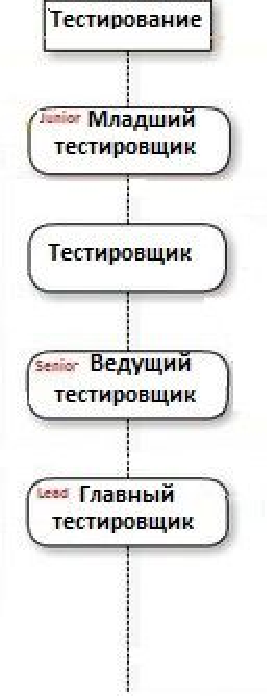
\includegraphics[width=0.27\linewidth]{11-IT-specialist's-way/sch11b.pdf}}
\end{frame}
\lecturenotes
 2ой~\cite{mc} прямой веткой  - является ветка внутри сегмента, связанного с тестированием. Далее рассмотрим подробнее


\begin{frame} \frametitle{Прямая ветка тестировщика:Младший тестировщик}
 \begin{block}{}
  \alert{Позиция --- Младший тестировщик (Junior QA)}

Должностные обязанности: 
  \end{block}
  \begin{itemize}
  \item Проведение ручного тестирования разделов приложения
  \item Создание и поддержка тест---кейсов
  \item Взаимодействие с другими подразделениями компании для организации эффективной работы
 \item Общение с ИТ---службами для разбора найденных ошибок
\item Документальное сопровождение деятельности
  \end{itemize}
\end{frame}

\lecturenotes
Позиция – Junior~\cite{hh} QA~\cite{itcf}
Должностные обязанности~\cite{rab}: 
•	проведение ручного тестирования разделов приложения;
•	создание и поддержка тест-кейсов;
•	Взаимодействие с другими подразделениями компании для организации эффективной работы.
•	Общение с ИТ-службами для разбора найденных ошибок.
•	Документальное сопровождение деятельности.

\begin{frame} \frametitle{Прямая ветка тестировщика:Старший тестировщик}
 \begin{block}{}
  \alert{Позиция --- Тестировщик (Middle QA)}

Должностные обязанности в отличии от младшего тестировщика: 
  \end{block}
  \begin{itemize}
  \item Проведение функционального и регрессивного тестирования, cоставление отчетов по итогам проведенного тестирования
  \item Анализ требований и ТЗ на предмет корректности
  \item Работа в системе баг---трекинга
  \end{itemize}
\end{frame}

\lecturenotes
Позиция – Middle~\cite{hh} QA~\cite{itcf}
Обязанности~\cite{rab}:
•	проведение функционального и регрессивного тестирования, cоставление отчетов по итогам проведенного тестирования;
•	анализ требований и ТЗ на предмет корректности;
•	работа в системе баг-трекинга.

\begin{frame} \frametitle{Прямая ветка тестировщика:Ведущий тестировщик}
 \begin{block}{}
  \alert{Позиция --- Ведущий тестировщик (Senior QA)}

Должностные обязанности в отличии от тестировщика: 
  \end{block}
  \begin{itemize}
  \item Постоянное взаимодействие с командой разработки
  \item Уточнение требований к ПО заказчика или бизнес---аналитиков
  \item Оценка возможных рисков
 \item Внедрение идей оптимизации рабочего процесса
 \item Обучение кадров
  \end{itemize}
\end{frame}

\lecturenotes
Позиция – Senior~\cite{hh} QA~\cite{itcf}

ЗАДАЧИ~\cite{rab}:
•	постоянное взаимодействие с командой разработки;
•	уточнение требований к ПО заказчика или бизнес-аналитиков;
•	оценка возможных рисков;
•	внедрение идей оптимизации рабочего процесса.
•	обучение кадров.


\begin{frame} \frametitle{Прямая ветка тестировщика:Главный тестировщик}
 \begin{block}{}
  \alert{Позиция --- Ведущий тестировщик (Lead QA)}

Должностные обязанности в отличии от ведущего тестировщика: 
  \end{block}
  \begin{itemize}
  \item Руководство работами по созданию тестовых спецификаций, подготовке к тестированию, проведению тестирования, составлению и обработке отчетов
  \item Отчетность перед менеджером проекта и начальником отдела о ходе выполнения поставленных задач
  \item Оценка возможных рисков
 \item Планировать работы по автоматизации тестирования
 \item Заниматься рефакторингом
  \end{itemize}
\end{frame}

\lecturenotes
Позиция – Lead QA~\cite{hh} (Главный тестировщик)~\cite{itcf}
Обязанности~\cite{rab}:
•	Руководство работами по созданию тестовых спецификаций, подготовке к тестированию, проведению тестирования, составлению и обработке отчетов.
•	Отчетность перед менеджером проекта и/или начальником отдела о ходе выполнения поставленных задач.
•	Планировать работы по автоматизации тестирования;
•	Заниматься рефакторингом;


\begin{frame} \frametitle{Прямая ветка автоматизация }
  \centerline{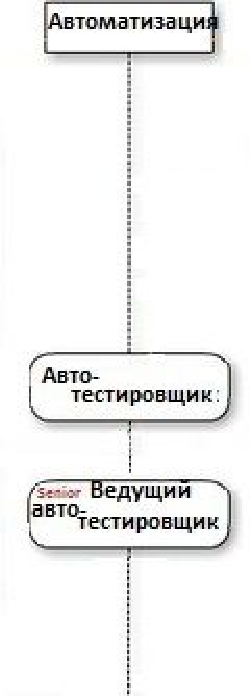
\includegraphics[width=0.27\linewidth]{11-IT-specialist's-way/sch11c.pdf}}
\end{frame}

\lecturenotes
 3ей~\cite{mc} прямой веткой  - является ветка внутри сегмента, связанного с автоматизацией. Далее рассмотрим подробнее

\begin{frame} \frametitle{Прямая ветка автоматизации: Авто-тестировщик }
 \begin{block}{}
  \alert{Позиция --- Старший авто-тестировщик ( Middle Automatization QA)}

Должностные обязанности в отличии от тестировщика: 
  \end{block}
  \begin{itemize}
  \item Разработка и поддержка специализированного фрэймворка для автоматизированного тестирования
  \item  Разработка тестов для определенной функциональности устройства по низкоуровневой документации на устройство
  \item Поддержка и запуск тестов в рамках системы автоматического автоматизированного тестирования и коммуникация с другими группами (в рамках и за пределами команды) в зависимости от результатов тестирования
 \item  Визуализация результатов тестирования и ее последующая автоматизация
  \end{itemize}
\end{frame}

\lecturenotes
Позиция – Авто~\cite{hh} тестировщик~\cite{itcf}
Задачи~\cite{rab}:
- Разработка и поддержка специализированного фрэймворка для автоматизированного тестирования.
- Разработка тестов для определенной функциональности устройства по низкоуровневой документации на устройство.
- Поддержка и запуск тестов в рамках системы автоматического автоматизированного тестирования и коммуникация с другими группами (в рамках и за пределами команды) в зависимости от результатов тестирования.
- Визуализация результатов тестирования и ее последующая автоматизация.

\begin{frame} \frametitle{Прямая ветка автоматизации: Ведущий авто-тестировщик }
 \begin{block}{}
  \alert{Позиция --- Ведущий авто-тестировщик ( Senior Automatization QA)}

Должностные обязанности в отличии от старшего авто-тестировщика: 
  \end{block}
  \begin{itemize}
  \item Обучение кадров
  \item  Участие в планировании направления деятельности
  \item Внедрении новых правил, методов работы и стандартов тестирования
 \item Координирование основной деятельности с внутренними отделами и внешними поставщиками
  \end{itemize}
\end{frame}

\lecturenotes
Позиция – Ведущий Авто~\cite{hh} тестировщик~\cite{itcf}
Задачи~\cite{rab}:
•	Обучение кадров
•	Участие в планировании деятельности направления
•	Внедрении новых правил, методов работы и стандартов тестирования
•	Координирование основной деятельности с внутренними отделами и внешними поставщиками

\begin{frame} \frametitle{Прямая ветка дизайна }
  \centerline{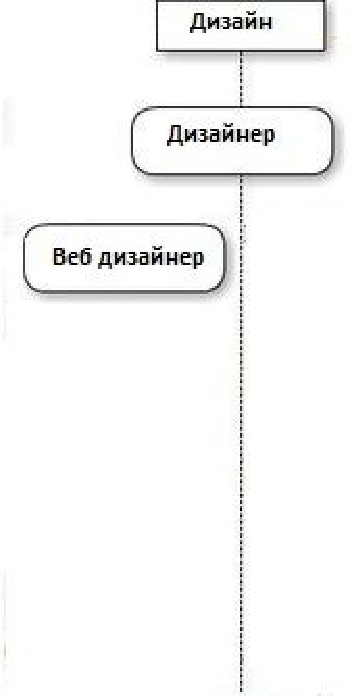
\includegraphics[width=0.27\linewidth]{11-IT-specialist's-way/sch11d.pdf}}
\end{frame}

\lecturenotes
 4ой~\cite{mc} прямой веткой  - является ветка внутри сегмента, связанного с дизайном. Данную ветка является неполной. В даннойчасти мы рассмотрим позиции - Дизайнер и Веб-дизайнер, а во второй части схемы рассмотри еще две позиции.

\begin{frame} \frametitle{Прямая ветка дизайна: Дизайнер }
 \begin{block}{}
  \alert{Позиция --- Дизайнер (Designer)}

Должностные обязанности: 
  \end{block}
  \begin{itemize}
  \item  Выполнение художественно-оформительских работ по заказам подразделений предприятия (клиентов)
  \item  Составление эскизов и согласовывание эскизов с непосредственным руководителем 
  \item Консультирует своего непосредственного руководителя (клиента) о принципах и вариантах решения поставленных дизайнерских задач
 \item  Вносит исправления в проекты художественного и технического оформления по указанию художественного редактора
  \end{itemize}
\end{frame}

\lecturenotes
Позиция~\cite{hh} – Дизайнер~\cite{itcf}
Должностные обязанности~\cite{rab}:
1.	Осуществляет своевременное и качественное выполнение художественно-оформительских работ по заказам подразделений предприятия (клиентов).
2.	Разрабатывает проекты художественного и технического оформления изданий исходя из информации, полученной от непосредственного руководителя или клиента (об адресной аудитории, о цели издания, о сроках выполнения, о требуемом качестве, пр.).
3.	Составляет эскизы и выполняет работы по художественному оформлению публикаций различного характера (в журналах, книгах, иных изданиях), проектов, отчетов, информационных и рекламных материалов; разрабатывает эскизы упаковки, товарных знаков, пр.
4.	Консультирует своего непосредственного руководителя (клиента) о принципах и вариантах решения поставленных дизайнерских задач.
5.	Согласовывает эскизы (проекты) с непосредственным руководителем (клиентом) и подготавливает окончательные макеты информационных изданий (пресс-релизов, объявлений, бюллетеней, ведомостей, прайс-листов, справочников, пр.), идентифицирующих материалов (визитных карточек, этикеток, упаковки, бланков, пр.), справочных изданий (адресных книг, учебных и иных пособий, пр.), художественно-публицистических изданий (книг, журналов, газет, пр.).
6.	Вносит исправления в проекты художественного и технического оформления по указанию художественного редактора.

\begin{frame} \frametitle{Прямая ветка дизайна: Веб дизайнер }
 \begin{block}{}
  \alert{Позиция --- Веб дизайнер (Web Designer)}

Должностные обязанности в отличии от дизайнера: 
  \end{block}
  \begin{itemize}
  \item   Разработка концепции дизайна и интерфейса web---сайта
  \item  Отрисовка дизайн---макетов (технический дизайн) разделов, страниц, интерфейсов, модулей
  \item Подготовка и размещение на сайте графики и контента
 \item Оптимизация дизайна существующих и разработка новых интерфейсов
  \end{itemize}
\end{frame}

\lecturenotes
Позиция – Веб~\cite{hh} Дизайнер~\cite{itcf}
Должностные обязанности web-дизайнера~\cite{rab}:
- разработка концепции дизайна и интерфейса web-сайта;
- отрисовка дизайн-макетов (технический дизайн) разделов, страниц, интерфейсов, модулей;
- создание графических и стилистических элементов для сайтов, дизайн баннеров и промостраниц, создание презентаций;
- подготовка и размещение на сайте графики и контента;
- оптимизация дизайна существующих и разработка новых интерфейсов.
- заполнение, продвижение и поддержка работы сайта,
- макетирование и верстка полиграфической продукции для внутреннего использования (бланки, буклеты, визитки).

\begin{frame} \frametitle{Косвенные ветки:1 часть из 4}
 \begin{block}{}
Косвенные ветки представленны 2 более крупными группами. Эти группы представляют собой набор навыков, необходимых для перехода от одной специальности к другой.
  \end{block}
  
\begin{block}{}
 \alert{Технические навыки} Переход: 

Веб дизайнер ---> Разработчик
  \end{block}

 \begin{block}{}
 \alert{Технические навыки} Переход: 

 Разработчик ---> Авто-тестировщик 

 Тестировщик --->  Авто-тестировщик
  \end{block}
\end{frame}


\begin{frame} \frametitle{Косвенные ветки:1 часть из 4, Подробнее}

\begin{block}{Веб дизайнер ---> Разработчик}

Возможно при дополнительном изучении:
  \end{block}
\begin{itemize}
  \item Изучение и понимание технологии web---серверов и приложений
  \item Изучение клиентских технологий, сред разработки
  \end{itemize}

 \begin{block}{Тестировщик ---> Авто-тестировщик        и 

Разработчик ---> Авто-тестировщик }

Возможно при дополнительном изучении:
  \end{block}
\begin{itemize}
  \item Разработка и поддержка специализированного фрэймворка для автоматизированного тестирования
  \item Запуск тестов в рамках системы автоматического автоматизированного тестирования
\item Визуализация результатов тестирования
  \end{itemize}
\end{frame}

\lecturenotes

Веб-дизайнер ---------Middle разработчик
Возможно при дополнительном изучении~\cite{rab}:
•	Software Engineering Process
•	 Изучение и понимание технологии web-серверов и серверов приложений
•	Изучение клиентских и серверных технологий , 
•	Изучение сред разработки


o	Тестировщик ---------Авто-тестировщик
Возможно при дополнительном умении:
•	Разработка и поддержка специализированного фрэймворка для автоматизированного тестирования.
•	Поддержка и запуск тестов в рамках системы автоматического автоматизированного тестирования и коммуникация с другими группами (в рамках и за пределами команды) в зависимости от результатов тестирования.
•	Визуализация результатов тестирования и ее последующая автоматизация.


o	Разработчик---------Авто-тестировщик
Возможно при дополнительном умении:
•	Разработка и поддержка специализированного фрэймворка для автоматизированного тестирования.
•	Поддержка и запуск тестов в рамках системы автоматического автоматизированного тестирования и коммуникация с другими группами (в рамках и за пределами команды) в зависимости от результатов тестирования.
•	Визуализация результатов тестирования и ее последующая автоматизация.


\begin{frame} \frametitle{Развитие  специалиста в иерархии компании: 2 часть из 4 }
  \centerline{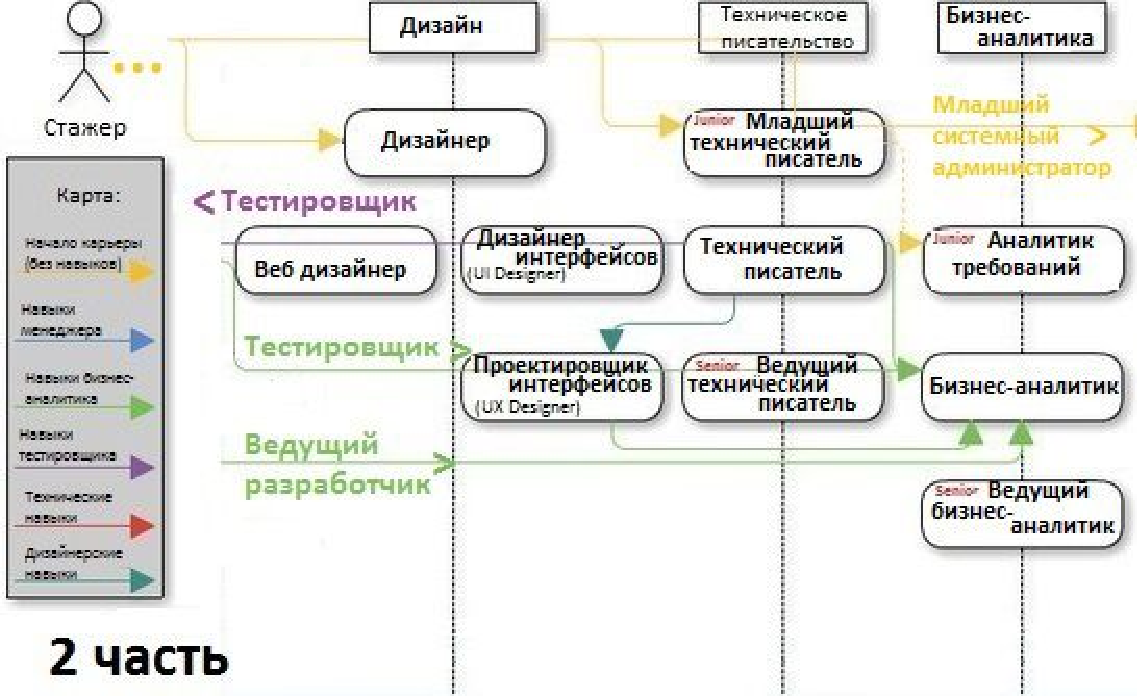
\includegraphics[width=1\linewidth]{11-IT-specialist's-way/sch12.pdf}}
\end{frame}

\begin{frame} \frametitle{Прямая ветка дизайна }
  \centerline{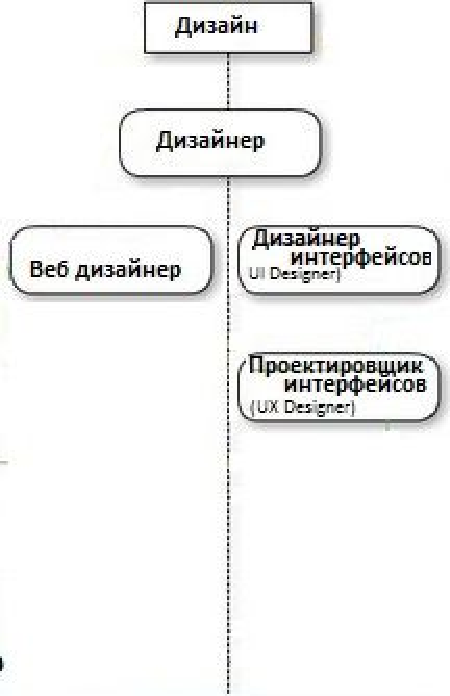
\includegraphics[width=0.42\linewidth]{11-IT-specialist's-way/sch12a.pdf}}
\end{frame}

\lecturenotes
 1ой~\cite{mc} прямой веткой  - является ветка внутри сегмента, связанного с дизайном. Полная ветка ветка,2 позиции были рассмотрены в предыдущей части.


\begin{frame} \frametitle{Прямая ветка дизайна: Дизайнер и проектировщик интерфейсов }
 \begin{block}{}
 Дизайнер интерфейсов(UI дизайнера) занимается  отрисовкой интерфейса на основе UX данных и ответственен за то, какие физические характеристики приобретет продукт.
  \end{block}
 \begin{block}{}
Проектировщик интерфейсов(UX дизайнера) проектирует интерфейс, который позволит достигать нужной цели в использовании продукта максимально простым и удобным путем.
  \end{block}
   \begin{block}{}
 UI и UX  --- это 2 разных профиля дизайна, но чаще всего задачи по обоим направлениям связаны, и их выполняет один универсальный специалист.
  \end{block}
\end{frame}

\lecturenotes
UX~\cite{hh}~\cite{itcf}  и UI — это 2 разных профиля дизайна, но чаще всего задачи по обоим направлениям тесно связаны между собой, а потому их выполняет один универсальный специалист.
Позиция –UX/UI дизайнер совмещает обе роли — проектирует, как пользователь будет взаимодействовать с интерфейсом и какие шаги ему нужно предпринять, чтобы сделать что-то (UX), а также определяет, как будет выглядеть каждый из этих шагов (UI).
•	позиция – UX Дизайнер
Аббревиатура UX расшифровывается как User eXperience и подразумевает, какой опыт/впечатление получает пользователь от работы с продуктом. Задача UX дизайнера — спроектировать такой интерфейс, который позволит достигать нужной цели в использовании продукта максимально простым и удобным путем.
•	позиция – UI Дизайнер
UI — это User Interface, визуальный вид продукта. Задача UI дизайнера — сделать интерфейс целостным, красивым и понятным. UI дизайнер занимается непосредственно отрисовкой интерфейса на основе UX данных и ответственен за то, какие физические характеристики приобретет продукт.
Для удобства далее будем рассматривать 2 данные позиции как одну.

\begin{frame} \frametitle{Прямая ветка дизайна: Дизайнер и проектировщик интерфейсов }
 \begin{block}{}
  \alert{Позиции --- Дизайнер интерфейсов (UI Designer) и Проектировщик интерефейсов (UX Designer)}

Должностные обязанности в отличии от дизайнера: 
  \end{block}
  \begin{itemize}
  \item   Сбор информации о проекте и его аудитории
  \item  Проектирование пользовательских сценариев
  \item Разработка стиля, составление инструкций по шрифтам, цветам и размерам
 \item Аудит юзабилити сайта с применением когнитивных измерений
  \end{itemize}
\end{frame}

\lecturenotes
Ключевые обязанности UX/UI дизайнера~\cite{rab}:
-сбор информации о проекте и его аудитории;
-проектирование пользовательских сценариев;
-разработка стиля, составление инструкций по шрифтам, цветам и размерам;
-создание макетов и прототипов;
-отрисовка интерфейса в графических редакторах.
-подготовка и передача макетов для разработчиков
-аудит юзабилити сайта с применением когнитивных измерений


\begin{frame} \frametitle{Прямая ветка технического писательства }
  \centerline{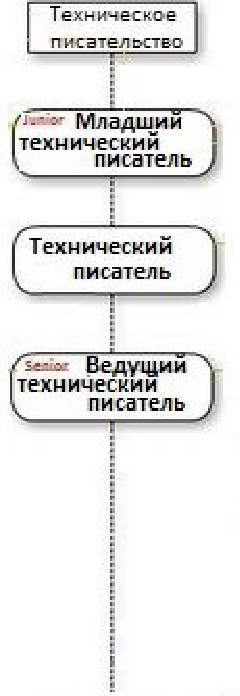
\includegraphics[width=0.27\linewidth]{11-IT-specialist's-way/sch12b.pdf}}
\end{frame}

\lecturenotes
 2ой~\cite{mc} прямой веткой  - является ветка внутри сегмента, связанного с техническим писательством. Подробнее разберем далее.


\begin{frame} \frametitle{Прямая ветка технического писательства: Младший технический писатель }
  \begin{block}{}
  \alert{Позиции --- Младший технический писатель (Junior TW) }

Должностные обязанности: 
  \end{block}
  \begin{itemize}
  \item  Разработка технической документации (руководств оператора и инженера, ПЗ, ТУ, ТЗ, технических паспортов и др.) в соответствии с требованиями
  \item  Проверка и корректировка технической документации
  \item Сбор информации у всех участников процесса: заказчиков, разработчиков, инженеров
 \item Владение ИТ---терминологией и техническим английским
  \end{itemize}
\end{frame}


\lecturenotes
Позиция – Junior Технический~\cite{hh} писатель~\cite{itcf}
Обязанности~\cite{rab}:
•	Разработка, проверка и корректировка технической документации (руководств оператора и инженера, правил эксплуатации, ПЗ, ТУ, ТЗ, технических паспортов и прочих документов) в соответствии с требованиями ГОСТ 
•	Подготовка графических схем по исходным данным
•	Сбор информации у всех участников процесса: заказчиков, разработчиков, инженеров
•	Подготовка материалов технических презентаций
•	Владение ИТ-терминологией и английским;

\begin{frame} \frametitle{Прямая ветка технического писательства: Технический писатель }
  \begin{block}{}
  \alert{Позиции --- Технический писатель (Middle TW) }

Должностные обязанности в отличии от младшего технического писателя: 
  \end{block}
  \begin{itemize}
  \item Корректировка технических заданий, формирование UseCase
  \item  Поддержание документации в актуальном состоянии
  \item Эпизодически обучение пользователей
 \item 	Согласование требований с отделом разработки
  \end{itemize}
\end{frame}


\lecturenotes
Позиция –  Технический~\cite{hh} писатель~\cite{itcf}~\cite{rab}
•	Участие в создании информационно-аналитических систем на всех этапах жизненного цикла;
•	Корректировка технических заданий, формирование UseCase;
•	Поддержание документации в актуальном состоянии
•	Эпизодически обучение пользователей;
•	Согласование требований с отделом разработки;

\begin{frame} \frametitle{Прямая ветка технического писательства: Ведущий технический писатель }
  \begin{block}{}
  \alert{Позиции --- Ведущий технический писатель (Senior TW) }

Должностные обязанности в отличии от технического писателя: 
  \end{block}
  \begin{itemize}
  \item Управление разработкой и оценка затрат на создание комплекта технической документации
  \item Поиск путей улучшения выпускаемой технической документации
  \item Внедрение в компании средств разработки технической документации
 \item 	 Техническая поддержка разработчиков технической документации
  \end{itemize}
\end{frame}

\lecturenotes
Позиция – Senior Технический ~\cite{hh} писатель~\cite{itcf}
Задачи~\cite{rab}:
•	оценка затрат на создание комплекта технической документации 
•	управление разработкой комплекта технической документации
•	поиск путей улучшения выпускаемой технической документации 
•	внедрение в компании средств разработки тех. документации 
•	 техническая поддержка разработчиков технической документации


\begin{frame} \frametitle{Прямая ветка бизнес-аналитики }
  \centerline{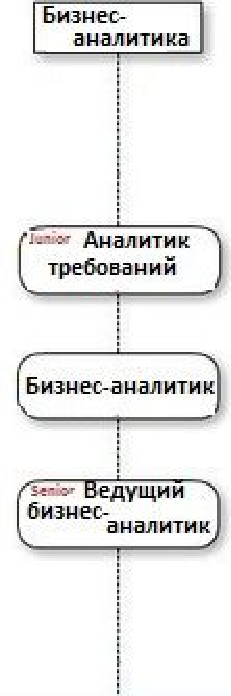
\includegraphics[width=0.27\linewidth]{11-IT-specialist's-way/sch12c.pdf}}
\end{frame}

\lecturenotes
 3ей~\cite{mc} прямой веткой  - является ветка внутри сегмента, связанного с работой бизнес-аналитиков. Подробнее разберем далее.

\begin{frame} \frametitle{Прямая ветка бизнес-аналитики:Аналитик требований }
  \begin{block}{}
  \alert{Позиции --- Аналитик требований (Junior  BA) }

Должностные обязанности: 
  \end{block}
  \begin{itemize}
  \item  Настройка бизнес---процессов в системе электронного документооборота 
  \item  Сбор и формализация требований Заказчика по автоматизации
  \item Участие в проектах по внедрению 
 \item Создание проектной документации
  \end{itemize}
\end{frame}


\lecturenotes
Позиция – Junior~\cite{hh} BA~\cite{itcf}
Обязанности~\cite{rab}:
•	Настройка бизнес-процессов в системе электронного документооборота 
•	Сбор и формализация требований Заказчика по автоматизации 
•	Участие в проектах по внедрению 
•	Создание проектной документации


\begin{frame} \frametitle{Прямая ветка бизнес-аналитики: Бизнес-аналитик}
  \begin{block}{}
  \alert{Позиции --- Бизнес-аналитик (Middle  BA) }

Должностные обязанности в отличии от аналитика требований: 
  \end{block}
  \begin{itemize}
  \item  Прогнозировать спрос,анализ отклонений от стратегических планов
  \item   Прогноз и оценка эффективности маркетинговой деятельности
  \item Оценка результатов продуктовых изменений и экспериментов
 \item  Сбор, обработка и хранение данных из CRM
 \item  Информационная поддержка руководителя
  \end{itemize}
\end{frame}


\lecturenotes
Позиция~\cite{hh} –  BA~\cite{itcf}

Обязанности~\cite{rab}:
	прогнозировать спрос 
⦁ Анализ отклонений от стратегических планов
⦁ Подготовка аналитических материалов, аналитических записок по деятельности компании
⦁ Прогноз и оценка эффективности маркетинговой деятельности
⦁ Оценка результатов продуктовых изменений и экспериментов
⦁ Анализ динамики статей консолидированной финансовой отчетности
⦁ Сбор, обработка и хранение данных из CRM
⦁ Информационная поддержка руководителя
⦁ Подготовка презентаций, работа с таблицами, графиками и т.д.


\begin{frame} \frametitle{Прямая ветка бизнес-аналитики: Ведущий бизнес-аналитик}
  \begin{block}{}
  \alert{Позиции --- Ведущий бизнес-аналитик (Senior  BA) }

Должностные обязанности в отличии от бизнес-аналитика: 
  \end{block}
  \begin{itemize}
  \item  Разработка и реинжиниринг бизнес---процессов компании
  \item   Экспертная поддержка проектов внедрения ИТ систем в части бизнес-процессов
  \item Способствование оптимальному функционированию системы управления качеством
 \item  Обеспечение исполнения решений руководства, своевременное информирование руководства о текущем ходе работ и их результатах
 \item  Обучение кадров
  \end{itemize}
\end{frame}


\lecturenotes
Позиция – Senior~\cite{hh} BA~\cite{itcf}
Обязанности~\cite{rab}:
•	Разработка и реинжиниринг бизнес-процессов в области:
− первичного производственного учета,
− расчета материального баланса,
− управления потерями и топливом на собственные нужды,
− повышения операционной эффективности.
•         обучение кадров
•	Экспертная поддержка проектов внедрения ИТ систем в части бизнес-процессов.
•	Участие в разработке технических требований и технических заданий для реализации ИТ инструментов автоматизации обновленных бизнес-процессов.  
•	способствование оптимальному функционированию системы управления качеством;
•	Обеспечение исполнения решений руководства, своевременное информирование руководства о текущем ходе работ и их результатах.






\begin{frame} \frametitle{Косвенные ветки:2 часть из 4}
 \begin{block}{}
Косвенные ветки представленны 3 более крупными группами
  \end{block}
  
\begin{block}{}
 \alert{Навыки аналитика} Переход: 

Тестировщик ---> Бизнес-аналитик

Ведущий разработчик ---> Бизнес-аналитик

Проектировщик интерфейсов ---> Бизнес-аналитик
  \end{block}

 \begin{block}{}
 \alert{Навыки дизайна} Переход: 

Технический писатель ---> Проектировщик интерфейсов
  \end{block}

\begin{block}{}
 \alert{Навыки тестирования} Переход: 

Технический писатель ---> Тестировщик
  \end{block}
\end{frame}


\begin{frame} \frametitle{Косвенные ветки:2 часть из 4, Подробнее}

\begin{block}{Тестировщик ---> Бизнес-аналитик  и

Ведущий разработчик ---> Бизнес-аналитик  и

Проектировщик интерфейсов ---> Бизнес-аналити}

Возможно при дополнительном изучении:
  \end{block}
\begin{itemize}
  \itemПодготовка аналитических материалов, аналитических записок по деятельности компании
  \item Прогноз спроса и оценка эффективности маркетинговой деятельности
\item Анализ динамики статей консолидированной финансовой отчетности
  \end{itemize}
\end{frame}

\lecturenotes
o	Тестировщик ---------Бизнес-аналитик
Возможно при дополнительном умении~\cite{rab}:

⦁ Подготовка аналитических материалов, аналитических записок по деятельности компании
⦁ Прогноз спроса и оценка эффективности маркетинговой деятельности
⦁ Оценка результатов продуктовых изменений и экспериментов
⦁ Анализ динамики статей консолидированной финансовой отчетности

o	Senior разработчик ---------Бизнес-аналитик
Возможно при дополнительном умении:
•	прогнозировать спрос 
⦁ Прогноз и оценка эффективности маркетинговой деятельности
⦁ Анализ динамики статей консолидированной финансовой отчетности

o	UX Дизайнер ---------Бизнес-аналитик
Возможно при дополнительном умении:
•	прогнозировать спрос 
⦁ Подготовка аналитических материалов, аналитических записок по деятельности компании
⦁ Прогноз и оценка эффективности маркетинговой деятельности
⦁ Анализ динамики статей консолидированной финансовой отчетности





\begin{frame} \frametitle{Косвенные ветки:2 часть из 4, Подробнее}

\begin{block}{Технический писатель ---> Проектировщик интерфейсов}

Возможно при дополнительном изучении:
  \end{block}
\begin{itemize}
  \item Принципов проектирования пользовательских сценариев
  \item Отрисовки интерфейса в графических редакторах
\item Подготовки и передачи макетов для разработчиков
  \end{itemize}

\begin{block}{Технический писатель ---> Тестировщик}

Возможно при дополнительном изучении:
  \end{block}
\begin{itemize}
  \item Принципов проведения ручного тестирования разделов приложения
  \item Создание тест-кейсов,проведение функционального и регрессивного тестирования
  \end{itemize}
\end{frame}

\lecturenotes
Технический писатель ---------UX Дизайнер
Возможно при дополнительном умении~\cite{rab}:
•	проектировать пользовательских сценариев;
•	отрисовка интерфейса в графических редакторах.
•	подготовка и передача макетов для разработчиков
•	разработка стиля, составление инструкций по шрифтам, цветам и размерам;


o	Технический писатель ---------Тестировщик
Возможно при дополнительном умении:
•	проведение ручного тестирования разделов приложения;
•	создание и поддержка тест-кейсов в актуальном состоянии;
•	проведение функционального и регрессивного тестирования, cоставление отчетов по итогам проведенного тестирования;
•	тестирование верстки страниц при различных сценариях поведения пользователей;
•	работа в системе баг-трекинга.




\begin{frame} \frametitle{Развитие  специалиста в иерархии компании: 3 часть из 4 }
  \centerline{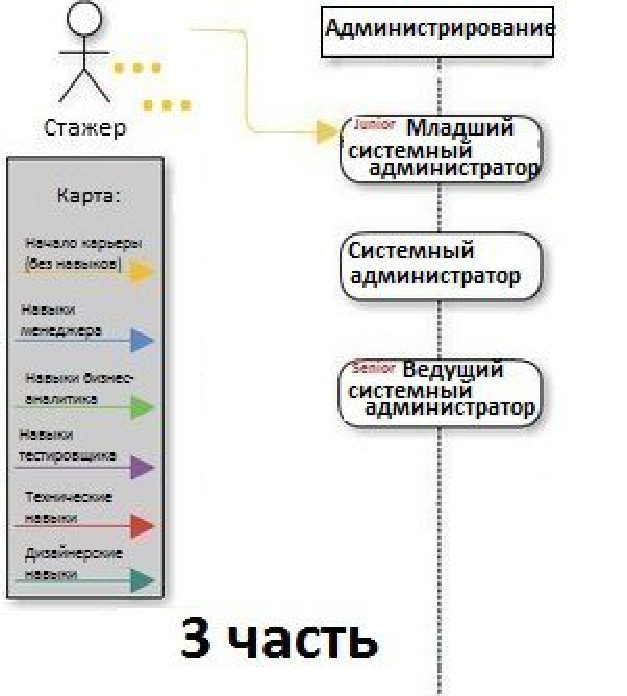
\includegraphics[width=0.62\linewidth]{11-IT-specialist's-way/sch13.pdf}}
\end{frame}


\begin{frame} \frametitle{Прямая ветка администрирования: Младший системный администратор }
 \begin{block}{}
  \alert{Позиция --- Младший системный администратор (Junior admin)}

Должностные обязанности: 
  \end{block}
  \begin{itemize}
  \item   Администрирование рабочих станций и решение проблем пользователя
  \item  Сопровождение ИТ оборудование удаленно
  \item Быстрое и полное восстановление данных при потери части или всей информации по вине любого из сотрудников;
 \item Сопровождение программных продуктов
 \item Обеспечение бесперебойной работы ИТ---инфраструктуры предприятия
  \end{itemize}
\end{frame}

\lecturenotes
Позиция – Junior системный~\cite{hh} админ~\cite{itcf}
Задачи~\cite{rab}:
•	Администрирование рабочих станций и решение проблем пользователя
•	Сборка, установка и настройка ПК
•	сопровождение ИТ оборудование удаленно
•	Сборка образов ОС Linux, Windows
•	Выполнение регламентных работ
•	Обслуживание, установка и переустановка офисной оргтехники, обеспечение ее высокопродуктивной деятельности
•	Поиск хорошего программного обеспечения, его установка, корректировка его деятельности; обеспечение постоянной бесперебойной работы сети компании
•	Быстрое и полное восстановление данных при потери части или всей информации по вине любого из сотрудников
•	Настройка, поддержка и модернизация локальной сети
•	Техническая поддержка пользователей
•	Сопровождение программных продуктов (таких как: 1С)
•	Обеспечение бесперебойной работы ИТ-инфраструктуры предприятия

\begin{frame} \frametitle{Прямая ветка администрирования: Старший системный администратор }
 \begin{block}{}
  \alert{Позиция --- Cистемный администратор (Middle admin)}

Должностные обязанности в отличии от младшего системного администратора: 
  \end{block}
  \begin{itemize}
  \item   Развёртывание, настройка и поддержание серверов, систем хранения данных, операционных систем и т.п.
  \item Навыки работы с виртуальными средами, контейнерными технологиями
  \item Обучение кадров
 \item Сопровождение программных продуктов
 \item Выявление потенциальных проблем, анализ текущей работы серверов и системного ПО
  \end{itemize}
\end{frame}

\lecturenotes
Позиция – Системный~\cite{hh} администратор~\cite{itcf}
Обязанности~\cite{rab}:
- развёртывание, настройка и поддержание серверов, систем хранения данных, операционных систем и т.п.
- навыки работы с виртуальными средами, контейнерными технологиями;
- Обучение кадров;
-выявление потенциальных проблем, анализ текущей работы серверов и системного ПО.

\begin{frame} \frametitle{Прямая ветка администрирования: Ведущий системный администратор }
 \begin{block}{}
  \alert{Позиция --- Ведущий системный администратор (Senior admin)}

Должностные обязанности в отличии от  системного администратора: 
  \end{block}
  \begin{itemize}
  \item   Руководство и планирование работы отдела
  \item  Разработка предложений по развитию инфраструктуры сети
  \item Подготовка предложений по модернизации и приобретению сетевого оборудования, в том числе участие в составлении технических заданий на закупку оборудования
  \end{itemize}
\end{frame}

\lecturenotes
Позиция – Senior Системный~\cite{hh} админ~\cite{itcf}

Обязанности~\cite{rab}:
•	Руководство и планирование работы отдела.
•	Разработка предложений по развитию инфраструктуры сети.
•	Подготовка предложений по модернизации и приобретению сетевого оборудования, в том числе участие в составлении технических заданий на закупку оборудования



\begin{frame} \frametitle{Развитие  специалиста в иерархии компании: 4 часть из 4 }
  \centerline{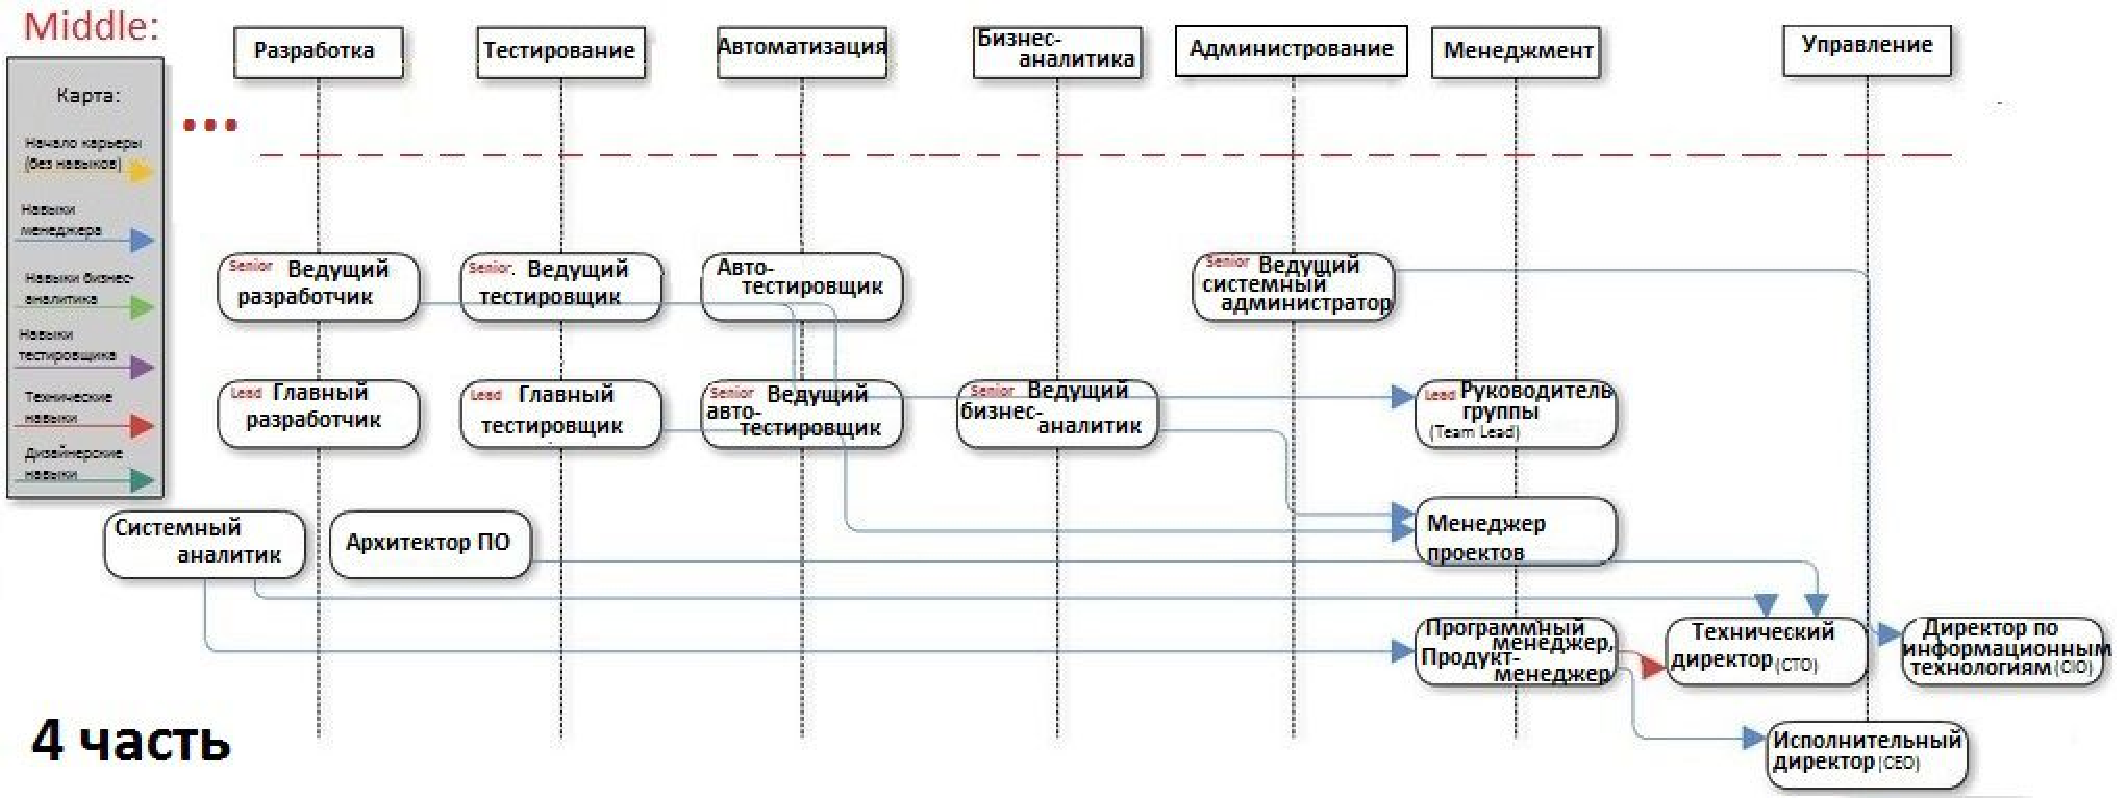
\includegraphics[height=0.53\textheight]{11-IT-specialist's-way/sch22.pdf}}
\end{frame}


\begin{frame} \frametitle{Прямая ветка управления}
  \centerline{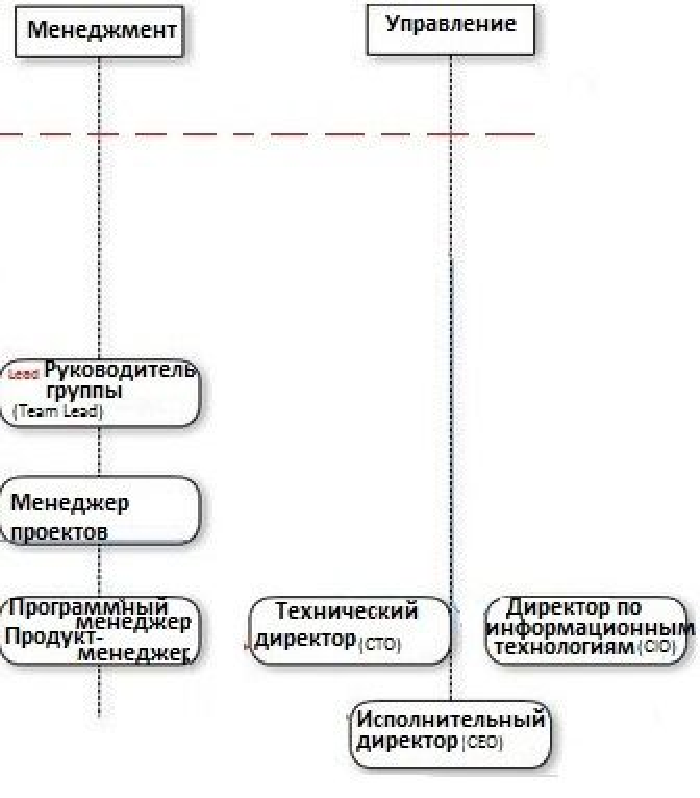
\includegraphics[width=0.63\linewidth]{11-IT-specialist's-way/sch22a.pdf}}
\end{frame}
\lecturenotes
 1 прямая~\cite{mc} ветка  -  менеджмент. Далее рассмотрим подробнее



\begin{frame} \frametitle{Прямая ветка управления: Руководитель группы}
 \begin{block}{}
  \alert{Позиция --- Руководитель группы (Team Lead)}

Должностные обязанности в отличии от Главных (разработчиков, тестировщиков, бизнес-аналитиков, системных администраторов и т.д.): 
  \end{block}
  \begin{itemize}
  \item Управление версиями проекта
  \item Подбор команды для реализации проекта,обучение персонала
 \item  Переговоры с клиентами, подготовка коммерческих предложений, проведение презентаций
  \item Составление отчетности для руководства
  \end{itemize}
\end{frame}

\lecturenotes
Позиция – Руководитель~\cite{hh} группы~\cite{itcf}

Обязанности~\cite{rab}:

- Управление отделом backend-разработки;
- Организация процесса разработки;
- Прототипирование;
- Разработка архитектуры системы;
- Трансформация use case/ spring tasks;
- Создание дизайн-моделей на базе т.з. и use case / user story;
- Написание API;
- Моделирование структуры хранения в базах данных
- Разработка функционала End-to-End;
- Code review;
- Документирование;
- Обучение членов команды.
- Организация взаимодействия с отделами аналитики, тестирования, администрирования;
- Unit - тесты;
- Ведение backlog;
- Управление версиями проекта;
- Подбор команды для реализации проекта;
- Переговоры с клиентами, подготовка коммерческих предложений, проведение презентаций;
- Составление отчетности для руководства;

\begin{frame} \frametitle{Прямая ветка управления: Менеджер проекта}
 \begin{block}{}
  \alert{Позиция --- Менеджер проекта (Project manager)}

Должностные обязанности в отличии от руководителя группы: 
  \end{block}
  \begin{itemize}
  \item Разработка плана управления проектом,детального дизайна
  \item Определение содержания проекта и разработка устава
 \item Планирование и управление рисками, контроль бюджета и сроков
  \item Мониторинг и управление работами проекта
  \end{itemize}
\end{frame}

\lecturenotes
Позиция –менеджер~\cite{hh} проектов~\cite{itcf}
Обязанности~\cite{rab}:
 • Разработка плана управления проектом;
• Разработка детального дизайна;
• Определение содержания проекта;
• Разработка устава проекта;
• Планирование и управление рисками;
• Управление изменениями проекта;
• Мониторинг и управление работами проекта;
• Контроль и управление качеством предоставляемых на проекте услуг;
• Контроль бюджета и сроков проекта;



\begin{frame} \frametitle{Прямая ветка управления: Программный менеджер, Продукт-менеджер}
 \begin{block}{}
  \alert{Позиции --- Продукт-менеджер (Product Manager)}

Должностные обязанности в отличии от менеджера проекта: 
  \end{block}
  \begin{itemize}
  \item Построение стратегии продвижения приложения на англоязычные рынки
  \item Управлять полным продуктовым циклом
 \item Определять цели и KPI, а потом достигать их вместе с командой
  \end{itemize}
\end{frame}

\lecturenotes

Позиция~\cite{hh} – продукт-менеджер~\cite{itcf}~\cite{rab}
•	Управление процессом развития стартап проекта 
•	Осуществление маркетингового анализа и исследований (изучение рынка, конкурентов и пр.).
•	Построение стратегии продвижения приложения на англоязычные рынки
•	Создание прототипов пользовательского интерфейса 
•	Управлять полным продуктовым циклом, совмещая роли product и project менеджера: искать и анализировать идеи, писать понятные технические задания, ставить задачи на разработку, расставлять приоритеты, планировать ресурсы, контролировать сроки и качество исполнения, анализировать полученные результаты;
•	Определять цели и KPI, а потом достигать их вместе с командой;



\begin{frame} \frametitle{Прямая ветка управления: Программный менеджер, Программный менеджер}
 \begin{block}{}
  \alert{Позиции --- Программный менеджер(program Manager)}

Должностные обязанности в отличии от менеджера проекта: 
  \end{block}
  \begin{itemize}
  \item Осуществляет выбор оптимального сочетания потребностей пользователей и возможностей информационной системы
 \item Управление заявками пользователей на обслуживание
 \item Осуществляет прогнозирование изменений в автоматизации предприятия и разрабатывает меры упреждающего управления
  \end{itemize}
\end{frame}

\lecturenotes

Позиция – программный~\cite{hh} менеджер~\cite{itcf}~\cite{rab}
1.	Осуществляет выбор оптимального сочетания потребностей пользователей и возможностей информационной системы.
2.	Разрабатывает методологическую основу информационной системы.
3.	Организует подготовку проектной документации, сметы расходов на информационную систему и ее функционирование.
4.	Руководит работами по настройке и поддержке информационной системы.
5.	Осуществляет:
1.	7.1. Контроль и установку программного обеспечения (software control & distribution).
2.	7.3. Управление заявками пользователей на обслуживание (incident management).
3.	7.4. Управление изменениями (change management):
o	управление запросами на изменения (RfC);
o	подтверждение и планирование изменений;
o	управление приоритетами запросов.
4.	7.5. Управление составом ИС (сonfiguration management):
o	контроль инфраструктуры посредством поддержки адекватных данных обо всех необходимых ресурсах;
o	предоставление текущего статуса и истории каждого элемента инфраструктуры;
o	взаимосвязь элементов инфраструктур.
5.	7.6. Управление надежностью (availability management).
6.	7.7. Устранение нарушений работы сервисов (problem management).
6.	Осуществляет прогнозирование изменений в автоматизации предприятия и разрабатывает меры упреждающего управления.


\begin{frame} \frametitle{Ветка управления:Директора}
 \begin{block}{}
  \alert{Позиции --- Технический директор(CTO)}

Должностные обязанности: 
  \end{block}
  \begin{itemize}
  \item Контроль выполнения плана производства; определение контрольных точек для осуществления контроля процесса производства; ритмичный выпуск продукции
 \item Разработка и согласование расчетов производственных мощностей, технологических планировок и  процессов, подборе, комплектации и модернизации оборудования производства
 \item Контролировать организацию и проведение работ в подчиненных подразделениях в соответствии с утвержденными технологическими регламентами, картами, схемами, обеспечивать технически правильную эксплуатацию оборудования 
  \end{itemize}
\end{frame}

\lecturenotes
Позиция –CTO, технический~\cite{hh} директор~\cite{itcf}
•	Обязанности~\cite{rab}:
Управление службами
o	Технологический отдел
o	ПДО
o	Служба механика
o	Производство
o	ОТК
•	Контроль выполнения плана производства; определение контрольных точек для осуществления контроля процесса производства; ритмичный выпуск продукции
•	Разработка и согласование расчетов производственных мощностей, технологических планировок и технологических процессов, подборе, комплектации и модернизации оборудования производства, в освоении новых технологий;
•	Разработка и внедрение производственных процессов с целью повышения производительности и качества выпускаемой продукции.
•	Составление инвестиционных планов по техническому обеспечению.
•	Внедрение современных стратегий сокращения издержек производства; Участие в разработке проектов, направленных на улучшение организации производства.
•	Организовывать рациональное использование производственных ресурсов: полное использование имеющихся мощностей, рациональная загрузка и уменьшение простоев оборудования;
•	Организовывать текущее производственное планирование, учет, составление и своевременное представление отчетности о производственной деятельности подчиненных подразделений, организовывать работу по правильному применению форм и систем заработной платы и материального стимулирования.
•	Организовывать контроль за внесением изменений, анализировать изменения на качество продукции;
•	Организовывать и обеспечивать подготовку производства к прохождению внутренних и внешних проверок.
•	Контролировать организацию и проведение работ в подчиненных подразделениях в соответствии с утвержденными технологическими регламентами, картами, схемами, обеспечивать технически правильную эксплуатацию оборудования и других основных средств
•	Координировать работу цехов и функциональных служб подчиненных подразделений, определять полномочия, должностные обязанности и ответственность подчиненного персонала.
•	Анализировать деятельность подчиненных подразделений и результаты анализа доводить до сведения генерального директора


\begin{frame} \frametitle{Ветка управления:Директора}
 \begin{block}{}
  \alert{Позиции --- Исполнительный директор(CEO)}

Должностные обязанности: 
  \end{block}
  \begin{itemize}
  \item Организация работ и взаимодействия всех подразделений компании
 \item Оперативное выполнение анализа деятельности
 \item Проверка правильности делопроизводства: смотрит за соблюдением норм экономического и юридического делопроизводства
  \item Выполняет поручения непосредственного руководителя --- генерального директора
  \end{itemize}
\end{frame}

\lecturenotes
Позиция –CEO, исполнительный~\cite{hh} директор~\cite{itcf}
Обязанности~\cite{rab}:
•	Организация работ и взаимодействия всех подразделений компании. 
•	Участие в развитии и стратегическом планировании деятельности предприятия. 
•	Оперативное выполнение анализа деятельности. 
•	Разработка системы мотивирующих стимулов для работников. 
•	Отвечает за соблюдение его подчиненными правил трудовой дисциплины. 
•	Проверка правильности делопроизводства: смотрит за соблюдением норм экономического и юридического делопроизводства.
•	 Выявляет недостатки в деятельности компании и предпринимает все возможные средства для устранения недостатков в работе. 
•	Выполняет поручения непосредственного руководителя - генерального директора. 


\begin{frame} \frametitle{Ветка управления:Директора}
 \begin{block}{}
  \alert{Позиции --- Директор по информационным технологиям(CIO)}

Должностные обязанности: 
  \end{block}
  \begin{itemize}
  \item Разработка модели монетизации проекта
 \item Постановка и распределение задач
\item Контроль сроков/стоимости/качества выполнения работ
 \item Разработка стратегии продвижения и рекламы продукта
  \itemМодернизация IT---инфраструктуры компании
  \end{itemize}
\end{frame}

\lecturenotes
	Позиция –CIO, Директор по информационным~\cite{hh} технологиям~\cite{itcf}

Обязанности~\cite{rab}:
- Разработка модели монетизации проекта;
- Оценка сроков и стоимости реализации системы;
- Разработка архитектуры развёртывания приложения;
- Разработка документации по проекту;
- Подбор исполнителей;
- Постановка и распределение задач;
- Контроль сроков/стоимости/качества выполнения работ;
- Организация непрерывного тестирования продукта;
- Разработка стратегии продвижения и рекламы продукта;
- Организация технической поддержки продукта.
- Подбор и обучение сотрудников;
- Модернизация IT-инфраструктуры компании.


\begin{frame} \frametitle{Косвенные ветки:4 часть из 4, Технические навыки}

\begin{block}{Программный менеджер ---> Технический директор  и

Продукт-менеджер ---> Технический директор }

Возможно, зазвивая технические навыки, при дополнительном изучении:
  \end{block}
\begin{itemize}
  \item Принципов создание, контроля и ведения плана производства
  \item Разработка и согласование расчетов производственных мощностей, технологических планировок и технологических процессов
\item Составление инвестиционных планов по техническому обеспечению
  \end{itemize}
\end{frame}

\lecturenotes
Программный менеджер, Продукт-менеджер ---------CTO (технический директор)
Возможно при дополнительном изучении~\cite{rab}:
 
•	Управление службами
o	Технологический отдел
o	ПДО
o	Служба механика
o	Производство
o	ОТК
•	Контроль выполнения плана производства; определение контрольных точек для осуществления контроля процесса производства; ритмичный выпуск продукции
•	Разработка и согласование расчетов производственных мощностей, технологических планировок и технологических процессов, подборе, комплектации и модернизации оборудования производства, в освоении новых технологий;
•	Составление инвестиционных планов по техническому обеспечению.
•	Организовывать и обеспечивать подготовку производства к прохождению внутренних и внешних проверок.
•	Анализировать деятельность подчиненных подразделений и результаты анализа доводить до сведения генерального директора


\begin{frame} \frametitle{Косвенные ветки:4 часть из 4, Навыки менеджера}

\begin{block}{Развивая навыки менеджера.}
Возможны переходы:
  \end{block}
\begin{itemize}
  \item Ведущий разработчик ---> Руководитель группы
  \item Ведущий тестировщик ---> Руководитель группы
\item Главный тестировщик---> Менеджер проекта
 \item Ведущий бизнес-аналитик ---> Менеджер проекта
  \item Архитектор ПО  ---> Технический директор
\item  Системный аналитик ---> Технический директор
 \item Системный аналитик ---> Программный менеджер, Продукт-менеджер
  \item Технический директор ---> Директор по информационным технологиям
\item  Программный менеджер, Продукт-менеджер  ---> Исполнительный директор
  \end{itemize}
\end{frame}




%\section{}

\section{Взаимосвязь интересов компании и интересов сотрудника. }

\subsection{}

\begin{frame} \frametitle{Вопросы, на которые компании и сотруднику важно получить ответы}
  \centerline{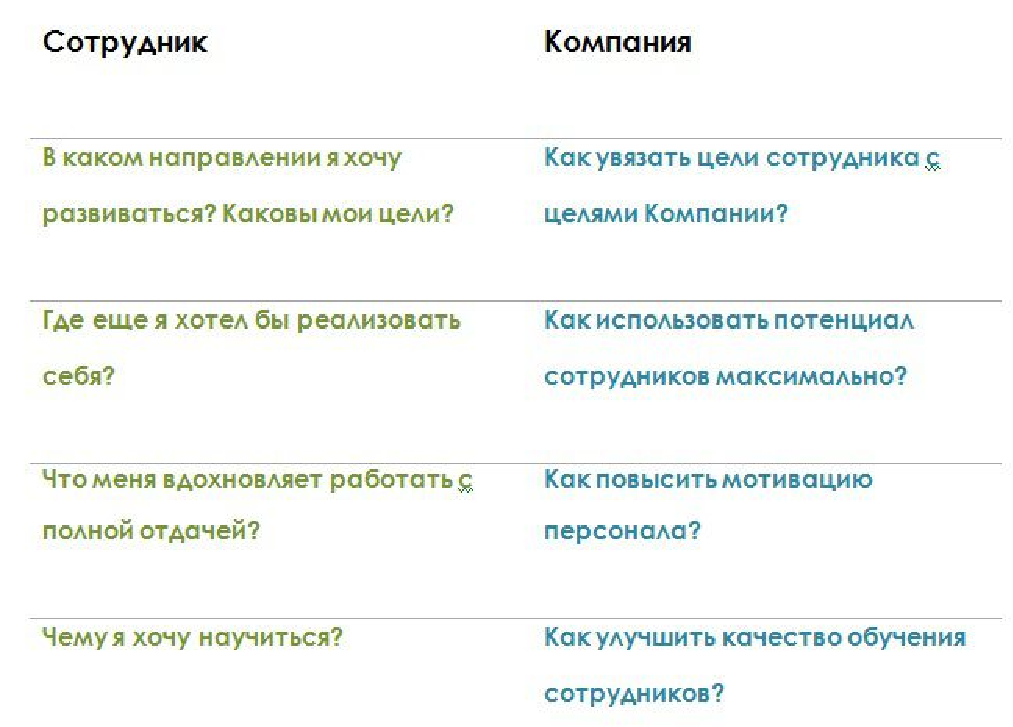
\includegraphics[height=0.82\textheight]{11-IT-specialist's-way/vop.pdf}}
\end{frame}


\lecturenotes
Вопросы~\cite{IPl}, на которые компании и сотруднику важно получить ответы(рисунок).
Для того чтобы ответить на вопросы представленные на картинке, важно понять, в чем состоит главный принцип удержания ценных сотрудников.


\begin{frame} \frametitle{Взаимосвязь интересов компании и интересов сотрудника}
  \begin{block}{Главный принцип удержания ценных сотрудников}
Удержать сотрудника можно, только объединив интересы Компании с интересами этого сотрудника
  \end{block}
  \centerline{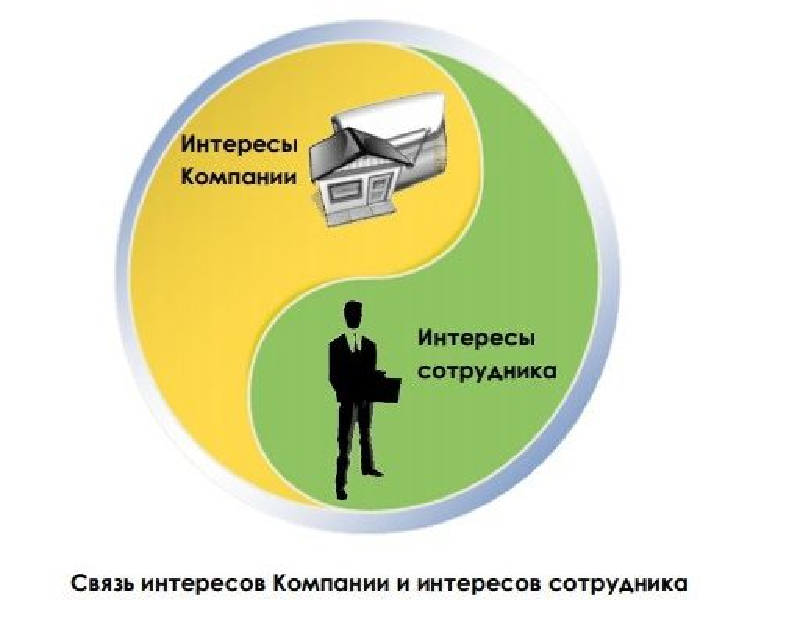
\includegraphics[height=0.58\textheight]{11-IT-specialist's-way/inter.pdf}}
\end{frame}

\lecturenotes
Главный~\cite{IPl} принцип удержания ценных сотрудников гласит, что удержать сотрудника можно, только объединив интересы Компании с интересами этого сотрудника.
Только при выполнение главного принципа удержания ценных сотрудников схемы мотивации компании будут работать, программы обучения действительно приносить приносить пользу и сотруднику и компании,а сам сотрудник будет стремиться расти и развиваться внутри конкретной компании.


%\section{}

\section{Индивидуальные планы развития сотрудников и компании. }

%\section{}

\begin{frame} \frametitle{Индивидуальные планы развития сотрудников и компании}
  \begin{block}{Индивидуальные планы развития}
 \alert{Индивидуальный план развития} – это современная эффективная технология развития ключевых сотрудников компании, которая обеспечивает максимальную согласованность интересов сотрудника с интересами Компании
  \end{block}
  
  \begin{block}{}
Результат напрямую зависит от умения правильно применять технологию
  \end{block}
\end{frame}

\lecturenotes
Индивидуальный план развития~\cite{IPl} – это современная эффективная технология развития ключевых сотрудников компании, которая обеспечивает максимальную согласованность интересов сотрудника с интересами Компании.

Как правило, индивидуальный план развития создается в диалоге между сотрудником и его руководителем. Однако это может быть также специалист по работе с персоналом Компании или приглашенный консультант. Результат напрямую зависит от умения правильно применять технологию.


\begin{frame} \frametitle{Индивидуальные планы развития сотрудников и компании}
  \begin{block}{Индивидуальные планы развития Сотрудника}
Дает сотруднику возможность стать активным участником процесса своего развития

План развития позволяет:
  \end{block}
  
   \begin{itemize}
  \item Понять четкие цели своего развития.
  \item Сосредоточить усилия в рамках выбранных направлений своего развития
  \item Оптимально использовать имеющиеся ресурсы
 \item Ускорить темп и повысить качество своего развития
  \end{itemize}
\end{frame}

\lecturenotes
Для сотрудника~\cite{IPl} индивидуальный план развития позволяет:

          Определить вектор своего профессионального и карьерного развития. Понять четкие цели своего развития. 
	Сосредоточить усилия в рамках выбранных направлений своего развития. 
	Оптимально использовать имеющиеся ресурсы (сотрудника и Компании) в процессе развития. 
	Ускорить темп и повысить качество своего развития. 

Но ГЛАВНОЕ, индивидуальный план развития дает сотруднику ВОЗМОЖНОСТЬ СТАТЬ АКТИВНЫМ УЧАСТНИКОМ процесса своего развития, влиять на него, самостоятельно оценивать личный прогресс и достижения. Это и означает – дать возможность своим ключевым сотрудникам реализовывать себя на все 100%.


\begin{frame} \frametitle{Индивидуальные планы развития сотрудников и компании}
  \begin{block}{Индивидуальные планы развития Компании}
Индивидуальные планы развития позволяют Компании раскрыть потенциал своих сотрудников максимально полно и направить его на решение бизнес---задач

План развития позволяет:
  \end{block}
  
   \begin{itemize}
  \item Связать цели развития сотрудника с целями Компании
  \item С учетом текущих возможностей и потребностей сотрудника выбирать подходящие задачи
  \item	 Планировать и проводить программы обучения с учетом реальных потребностей сотрудников 
  \end{itemize}
\end{frame}

\lecturenotes
Для Компании~\cite{IPl} индивидуальные планы развития позволяют:

	Связать цели развития сотрудника с целями Компании. Таким образом, достигая целей своего развития, сотрудник одновременно работает на достижение ключевых бизнес-показателей. В результате обеспечивается двойной полезный эффект – для сотрудника и для самой Компании.

	С учетом текущих возможностей и потребностей сотрудника выбирать подходящие задачи. Благодаря этому сотрудник становится заинтересованным в выполнении работы, прикладывает дополнительные усилия, а также развивается в процессе достижения цели. В результате Компания получает целеустремленного, растущего сотрудника, с готовностью решающего поставленные задачи.

	Планировать и проводить программы обучения с учетом реальных потребностей сотрудников. В итоге возрастает не только практическая эффективность обучения, но и повышается его ценность для сотрудников. Зачастую снижаются и расходы на обучение, потому что оно становится более дифференцированным – Вы перестает учить всему подряд.


Но ГЛАВНОЕ, индивидуальные планы развития позволяют Компании РАСКРЫТЬ ПОТЕНЦИАЛ своих лучших сотрудников максимально полно и НАПРАВИТЬ ЕГО НА РЕШЕНИЕ ВАЖНЕЙШИХ БИЗНЕС-ЗАДАЧ.

\begin{frame} \frametitle{Содержание индивидуальных планов развития}
  \begin{block}{ }
Индивидуальные планы развития представляет из себя документ, как правило, формирующийся в табличном виде и содержащий в себе:

  \end{block}
  
   \begin{itemize}
  \item Цели развития
  \item Мероприятия по развитию
  \item	 Указание лиц, ответственных за проведение этих мероприятий
 \item	Сроки проведения мероприятий
 \item	Отметки о выполнении
  \end{itemize}
\end{frame}

\lecturenotes
Индивидуальные планы~\cite{IPlan} развития представляет из себя документ, как правило, формирующийся в табличном виде и содержащий в себе:

  Цели развития.
 Мероприятия по развитию.
  Указание лиц, ответственных за проведение этих мероприятий.
 Сроки проведения мероприятий.
Отметки о выполнении.

\begin{frame} \frametitle{Когда составляются индивидуальные планы развития }
  \begin{block}{ }
Чаще всего составляется в следующих ситуациях:

  \end{block}
  
   \begin{itemize}
  \itemСотрудник только что принят на работу
  \item Сотрудник определен в кадровый резерв на вышестоящую должность
  \item	 Сотрудник демонстрирует недостаточно удовлетворительные результаты в работе
 \item	Составление плана развития находится в рамках бизнес---процесса по управлению результативностью
  \end{itemize}
\end{frame}

\lecturenotes
Чаще всего~\cite{IPlan} индивидуальный план развития составляется в следующих ситуациях:

1 Сотрудник только что принят на работу, необходимо упорядочить процесс его ввода в должность, адаптации к работе. В этом случае план развития чаще всего содержит в себе набор стандартных мероприятий, обусловленных не особенностями нового сотрудника, а требованиями конкретной должности.
2 Сотрудник определен в кадровый резерв на вышестоящую должность, необходимо планирование перспективного освоения функционала будущей должности. Чаще всего данный план представляет собой набор мероприятий по развитию управленческих компетенций.
3 Сотрудник демонстрирует недостаточно удовлетворительные результаты в работе, необходимо точечное развитие его компетенций. План развития формируется по результатам аттестации или деловой оценки сотрудника, представляет собой набор развивающих мероприятий, которые необходимо осуществить до повторной аттестации или деловой оценки.
4 Составление индивидуального плана развития сотрудника находится в рамках бизнес-процесса по управлению результативностью (Performance Management), внедренного в данной компании, осуществляется в обязательном порядке на ежегодной основе, и предназначено для согласования целей развития сотрудника с целями развития подразделения и компании в целом. Индивидуальный план развития формируется в процессе встречи сотрудника с непосредственным руководителем, в ходе которой сотрудник получает обратную связь об эффективности своей работы за год и выполнении предыдущих целей по развитию, в процессе совместного обсуждения согласуется постановка целей на будущий год. Как правило, данное мероприятие имеет влияние на результаты бонусирования сотрудника по итогам прошедшего года, а также может влиять на определение принципов бонусирования в будущем году.


%\section{}
\lecturenotes

Текст конспекта, относящийся к слайду с указанием источника~\cite[с.~97--99]{Brooks}.

На интернет-источники можно ссылаться не по ГОСТу, но с обязательной гиперссылкой~\cite{Fowler}.

\begin{thebibliography}{99}
\bibitem{Sonmez} Сонмез Джон Путь программиста.Человек эпохи ИТ. СПб~: Питер, 2016.
\bibitem{mc} \href{https://dou.ua/lenta/columns/karta-kariery/?from=foo}{ Карта карьеры.}
\bibitem{itcf} \href{https://www.itcareerfinder.com/it-careers.html}{ IT Careers.}
\bibitem{hh} \href{https://hh.ru}{ Вакансии. }
\bibitem{rab} \href{https://www.rabotka.ru/job_description/}{ Должностные инструкции. }
\bibitem{JMSL} \href{http://www.dataart.ru/news/junior-middle-senior-lead-etc-v-chem-raznitsa/}{ Сергей Марков Junior, Middle, Senior, Lead.}
\bibitem{IPl} \href{http://www.e-reading.club/chapter.php/1050422/98/Beron_-_Upravlenie_rezultativnostyu.html}{ Составление индивидуального плана развития.}
\bibitem{IPlan} \href{http://www.sbsc.ru/books/TalentWarBook.pdf}{ Составление индивидуального плана развития.}
\end{thebibliography}

\end{document}

%%% Local Variables: 
%%% mode: TeX-pdf
%%% TeX-master: t
%%% End: 
